\chapter{Methods}
\label{sec:methods}
This chapter explains the generation and preparation of the dataset and the implementation of the neural network architecture for classifying objects depending on their color feature.
The input consists of multiple views of an object, while percentages of class memberships are outputted.
The creation of the dataset is supported by the Blender API interface, while the model is written in Python using the tensorflow framework.

\section{Dataset Generation}
\label{sec:methods-dataset-generation}

\subsection{Choosing a Dataset}
\label{sec:dataset-choosing}
One requirement of the dataset is, that there are multiple views of the same object available.
Optimally, these views can be arbitrarily chosen for having as much freedom as possible for training and evaluating the network.
Hence, three-dimensional objects are necessary.
The related object categories are preferably discriminative to each other due to the objective of classifying real-world objects and easier evaluation of the model.
This means the dataset should not contain only flowers or faces for example.
These constraints bring up two possibilities.
The first one is creating new CAD objects.
These can be modeled in a way that supports the own needs the most.
However, creating plenty of models for every category would take a huge amount of time.
The second option is to use CAD models of an existing dataset.
Referring to the first possibility, this one just takes the time for finding a suited dataset and perhaps some slight modifications.
The time for manipulating this one according to the wanted color features compared to the self-created one is probably identical and, therefore, not taken into account.
Another advantage is the competitive ability because if this one is a popular dataset, other researches probably used it as a benchmark for their neural network as well.
Hence, a qualitative evaluation would be possible.
Taking all these arguments into account, an existing dataset is the best choice.

There are three different techniques for building a three-dimensional shape.
One uses triangles, where each one is defined by the position of its edges.
These positions are called vertices and contain an $x$-, $y$- and $z$-coordinate.
Additionally, each triangle has a normal vector and other information like a color and a texture.
Combining several triangles results in the final shape that is called a mesh object.
Another one uses voxels.
This word is a portmanteau of "volume" and "pixel" and represents a cell in a three-dimensional grid.
Each voxel behaves like a pixel and has a color.
The last technique is the point cloud.
Each point is represented by a vertex.
Such a cloud is often created by 3D scanners that measure a large number of points in a scene, like distances and sometimes color for digitalizing it.
A comparison of these techniques yields that the mesh object is the best-suited one.
It has the smoothest surface because it is continuous, hence, representing real-world objects most likely.
Using enough voxels could result in a similar shape, but the data size would be much bigger.
Furthermore, applying a color feature to a single triangle is easier than applying it to several voxels, where connected ones need to be found first.

The most popular dataset containing CAD objects in polygon mesh representation is ModelNet\cite{conf/cvpr/WuSKYZTX15}.
It contains 127,915 CAD models divided into 662 object categories for now.
For convenience, there are a 10-class and 40-class subset containing 10 or 40 popular categories, respectively.
Both are cleaned in respect to a wrong category sorting and then split into a training and a testing set.
Furthermore, the orientations of the models of the first one are aligned as well.
\subsection{Rendering Views of CAD Models}
\label{sec:dataset-rendering}
The following explains how multiple viewing perspectives of a single model are generated.
The properties of each CAD model of ModelNet are stored in a file that is loaded and interpreted in Blender.
To be able to refer to faces they are all part of the same basic coordinate system and are placed according to their defined vertices.
Because all models are oriented beforehand, their top points along the $z$-axis.
The origin of this coordinate system is set to the center of mass depending on the face areas.
For adding lighting to the object a lamp needs to be placed inside that coordinate system.
Blender offers several lamp types, but the Hemi lamp was chosen because it emits light radially from a plane.
Therefore, a homogeneous illumination is ensured.
%\begin{figure}
%	\centering
%	\begin{subfigure}{0.19\textwidth}
%		\centering
%		\includegraphics[width=\textwidth]{images/point.png}
%		\caption{Point}
%	\end{subfigure}
%	\begin{subfigure}{0.19\textwidth}
%		\centering
%		\includegraphics[width=\textwidth]{images/sun.png}
%		\caption{Sun}
%	\end{subfigure}
%	\begin{subfigure}{0.19\textwidth}
%		\centering
%		\includegraphics[width=\textwidth]{images/spot.png}
%		\caption{Spot}
%	\end{subfigure}
%	\begin{subfigure}{0.19\textwidth}
%		\centering
%		\includegraphics[width=\textwidth]{images/hemi.png}
%		\caption{Hemi}
%	\end{subfigure}
%	\begin{subfigure}{0.19\textwidth}
%		\centering
%		\includegraphics[width=\textwidth]{images/area.png}
%		\caption{Area}
%	\end{subfigure}
%	\caption[Lamp types available in Blender]{Lamp types available in Blender. Each light source is placed above the cube pointing directly towards it.}
%	\label{fig:blender-lamps}
%\end{figure}
Because all models have different heights and this type of lamp has no decay of intensity, it is placed above the objects far away from their origins.
By assigning the lamp a direction $\vec{r}_l = (0,0,0)^T$ it emits light along the negative $z$-axis directly onto the model.

For rendering views, a camera object is required.
Its parameters are left to the default values, except its view distance, which is set very high to work with all models.
Hence, only its location and rotation needs to be set.
Following the approach from \cite{Su:2015:MCN:2919332.2919750, Su2018} the camera is elevated 30 degrees from the ground plane and points towards the origin.
This results in the first rotation vector
\begin{equation}
	r_{c,0} = \left( \frac{r_{x,\text{deg}} \cdot \pi}{180}, 0, 0 \right)^T = \left( \frac{60 \cdot \pi}{180}, 0, 0 \right)^T
\end{equation}
in radians, where $r_{x,\text{deg}}$ is the rotation around the $x$-axis in degrees.
The first, second and third element define a rotation around the $x$-, $y$- and $z$-axis, respectively.
Because the camera points along the negative $z$-axis in its own coordinate system by default, $r_{x,\text{deg}} = 60$ corresponds to the mentioned setup.
The next step is fitting the camera view to the model just by changing the location of the camera.
Because Blender fits the camera view exactly to the object, an image padding is necessary for having empty border regions for later convolutions.
This is achieved by moving the camera away from the object along the line of their centers, i.\,e. along the negative view direction.
It is moved by
\begin{equation}
	\Delta d = \frac{d}{10}
\end{equation}
where $d$ is the distance from the mesh origin to the camera.
The advantage of a fraction is, that the padding is independent of the model's size.
Finally, this camera view is rendered with the following properties.
The resolution is defined to be $224 \times 224$ pixel
Furthermore, it needs to be coped with aliasing.
Because every pixel can only have a single color, diagonal lines usually have a step pattern.
This is not realistic, hence, it is smoothed out by anti-aliasing techniques.
This works by rendering the related image region in a higher resolution, taking several samples of pixel values and averaging them to get the value of the pixel in the desired resolution.
The best available sample size in Blender is 16, hence, it is chosen.
The background color is left at the default RGB color $\vec{c} = (64, 64, 64)$ resembling a dark gray for adding some noise to the views.
A black background would yield pixel intensities of 0 and resembles, in general, no real-world views.
Finally, this view is saved as a PNG file.
For gathering multiple views, the camera needs to be repositioned.
Hence, the following steps are repeated for the desired number of views.
The rotation of the camera is set to
\begin{equation}
	\vec{r}_c(v_i) = \left(  \frac{60 \cdot \pi}{180}, 0, \frac{v_i \cdot \varphi \cdot \pi}{180} \right)^T
\end{equation}
where $v_i$ is the view index, originally starting at 0, and $\varphi$ the moving interval in degrees.
The latter is set to
\begin{equation}
	\varphi = \frac{360}{n_v} = \frac{360}{12} = 30
\end{equation}
where $n_v$ equals the number of views.
For the ability to compare this work to related researches, $n_v = 12$ is defined.
The number of objects per set corresponds to \cite{Su:2015:MCN:2919332.2919750}.
That means, 90 objects per category class for the training set and 30 for the test set.
This process is repeated for each CAD object.
\subsection{Applying Material Feature Manipulations}
\label{sec:dataset-material-feature}
The objective is to clone every model and apply a color feature to every clone to be able to distinguish the same models.
Cloning is a trivial task because this can be done by rendering the native object first and then the color featured one.
One method for the color feature manipulation is preparing a color feature like a colored circle as an image and putting it on the model.
This feature can be scaled dependently on all the face areas for achieving a similar scale across all models.
However, clinging this image to a model considering all its edges is problematic.
It would be necessary to find a way to unfold the model along its edges.
This can be done by hand but is very time-consuming and complex.
In fact, Blender supports an automatic way of unfolding, but its results are not satisfying.
Therefore, this approach is not further pursued.
Another method is to color vertices.
However, for achieving reasonable features, a high number of vertices is necessary.
There is an option to subdivide existing faces and add additional vertices, but this increases the data size extremely, which needs much more computer performance and has the risk of inducing unwanted geometry into the model.
Hence, coloring single faces becomes the chosen approach due to its simplicity.
In CAD modeling objects are assigned a material with a color that reacts to light which produces shadows.
In Blender, the default material's color is a slightly darkened white.
Changing the color of a face is performed by changing the color of its material.

For following this approach, it is advisable to pre-define material presets.
Those presets consist of the default material but have different colors.
After making those presets available to the Blender scene, a well-suited face for being colored needs to be found.
In the following those faces are referred to as an optimal face.
It is important to filter all faces of an object by their area size.
\figref{fig:face-area-filter} shows why and the results of several thresholds.
\begin{figure}
	\centering
	\begin{subfigure}{.32\textwidth}
		\centering
		\includegraphics[width=\textwidth]{images/face_area_unfiltered.png}
		\caption{Unfiltered}
		\label{fig:face-area-unfiltered}
	\end{subfigure}
	\begin{subfigure}{.32\textwidth}
		\centering
		\includegraphics[width=\textwidth]{images/face_area_mean.png}
		\caption{Face Area Mean}
		\label{fig:face-area-mean}
	\end{subfigure}
	\begin{subfigure}{.32\textwidth}
		\centering
		\includegraphics[width=\textwidth]{images/face_area_max_dependent.png}
		\caption{Max Face Area Dependent}
		\label{fig:face-area-max-dependent}
	\end{subfigure}
	\caption{Threshold Setup for Filtering Faces by their Area Size}
	\label{fig:face-area-filter}
\end{figure}
If faces are not filtered at all, any face can result in being the optimal one.
However, it is not guaranteed that this face has a decent size and can be seen and recognized by the network easily.
This assumption was later verified by a not changing loss value during training.
Like in \figref{fig:face-area-unfiltered} the optimal face is comparatively small to the whole model.
Accepting only faces as the optimal face, that have at least the size of the mean of all faces lead to a result like in \figref{fig:face-area-mean}.
The optimal face can be seen more easily than before, but this threshold often results in long and slender optimal faces.
This is due to the fact, that the chosen object categories mostly contain objects that are built using such faces because they have longish surfaces.
Hence, filtering by the mean of the faces amplifies the probability to choose such a face as an optimal one.
Therefore, a threshold of above the mean is desired to skip all those lathy faces like it is shown in \figref{fig:face-area-max-dependent}.
Additionally, larger faces should be preferred.
Thus, the area of the optimal face have to satisfy
\begin{equation}
	a_{opt} > (a_{mean} + a_{max}) \cdot s
\end{equation}
where $a$ are the related areas and $s$ a scalar.
With $s = 0.3$ satisfying results are achieved.

Furthermore, it needs to be guaranteed, that the optimal face is visible in at least one view and not visible in at least one view.
This is validated by casting rays from the camera center onto the possible optimal face for every camera position that was defined in \secref{sec:dataset-rendering}.
In brief, if the rays hit the face, the face is visible.
Fortunately, there is a function in Blender performing this approach and returning among others the index of the face that is hit.
However, this cannot be performed for every pixel of a face due to performance issues.
Thus, the trade-off against accuracy is only checking the vertices defining the face.
This can raise errors, though, because a vertex can define multiple faces and it is not certain which face index the function returns.
Hence, each checkpoint $\vec{p}_i$ is moved slightly to the center of the face by
\begin{equation}
	\vec{p}_i = \vec{v}_i + 0.05 \cdot (\vec{f}_0 - \vec{v}_i)
\end{equation}
where $\vec{v}_i$ is the related vertex and $\vec{f}_0$ the center of the face.
If the ray cast is valid for at least one checkpoint the face is supposed to be visible.
If all rays hit the wrong face, the current face is supposed to be not visible.
As soon as both conditions are satisfied for the examined face among all views, it becomes the optimal face.
Otherwise, the next possible face is investigated.
If the conditions are never satisfied for each possible face, the object is skipped at all.

It is found, that a single optimal face is not enough, because some models have several duplicated faces.
Those are different faces where the coordinates of all the describing vertices are identical to the ones of other faces.
Hence, there are faces laying into each other.
This results in rendering issues like it is shown in \figref{fig:optimal-face}, because the rendering engine does not know, which material should be rendered on the surface.
In \figref{fig:optimal-face-single} only one of two identical faces is colored, which leads to the noticeable transparency effect.
That is one of the brighter effects, though.
It is also possible that one optimal face is shown normally and only on the edge rendering issues are visible like a dotted line with the colors of all optimal faces. 
Nevertheless, any of these effects could induce false correlations into the dataset that are not available on real-world objects, hence, leading to a not practical network.
Thus, in \figref{fig:optimal-face-all} the materials of all identical faces are changed, which leads to realistic color representations.
\begin{figure}
	\centering
	\begin{subfigure}{.49\textwidth}
		\centering
		\includegraphics[width=.7\textwidth]{images/optimal_face_single.png}
		\caption{Single Optimal Face}
		\label{fig:optimal-face-single}
	\end{subfigure}
	\begin{subfigure}{.49\textwidth}
		\centering
		\includegraphics[width=.7\textwidth]{images/optimal_face_all.png}
		\caption{All Optimal Faces}
		\label{fig:optimal-face-all}
	\end{subfigure}
	\caption{Material Manipulation on Duplicated Optimal Faces}
	\label{fig:optimal-face}
\end{figure}

Regarding a validation of the later model, an examination of two material features per object would be interesting.
Hence, for applying another material change on a model, another optimal face or faces, respectively, needs to be found.
A requirement for this is the presence of only one material feature in a single view.
Due to the automation of this task, a reliable solution is necessary.
One approach would be using the other side of the surface of the first optimal face.
However, this fails if the surface has a thickness of more than a single face.
Then the next face along its normal needs to be found by ray casting and then the visibility of this face needs to be verified.
Thus, this process leads to excessive ray cast validations and therefore not followed up on.
However, it is considered, that faces at a similar location as the original optimal face are well-suited as well.
Thus, the choices of further optimal faces are narrowed down by sorting all remaining faces by their distance from their center to the center of the first optimal face in descending order.
The intention is that choosing faces with the largest distances result in either a kind of opposite face or in a face that is that far away to not be visible at the same time. as the first optimal face.
Of course, the tasks of checking the visibility and finding identical faces are performed on the new face as well.
If no additional optimal face is found, the model is skipped, although, this never happened during execution.
\section{Preparing the Dataset}
\label{sec:methods-prepare-data}

\subsection{Single-View to Multi-View Conversion}
\label{sec:prepare-data-view-conversion}
The objective of the network is to classify multi-views of objects.
This means each input represents an object with all its corresponding views.
However, the views created in \secref{sec:dataset-material-feature} exist in single view representation because they are rendered successively.
Thus, each model's single views need to be converted into a related multi-view representation.
For achieving this, all single views are collected in order of their creation for keeping their relation.
Each view's pixel values are read, normalized to a range between 0 and 1, flattened to a vector $\vec{x}^{(i)}$ and stored in the input matrix $\vec{X}_{\text{set}}$ of the corresponding set.
Simultaneously to the view gathering each one-hot encoded label $\vec{y}^{(i)}$ needs to be created as well and put into the label matrix $\vec{Y}_{set}$ of the corresponding set similar to the views.
Each label may contain an object class, the so-called category, and a color mark class, the so-called color.
Depending on the type of classification, these two classes possibly need to be combined.
The single-label classification case embraces the following configurations.
If categories and colors are classified, both classes are appended to each other.
This results in $n_y = n_c \cdot n_m$ classes for classification, where $n_c$ is the number of categories and $n_m$ the number of color marks.
If only categories or color marks are classified, the final label contains only the category class or the material class, respectively.
Logically, the number of classes for classification, is either $n_y = n_c$ or $n_y = n_m$.
In the multi-label classification case, both labels are used independently.
Hence, the number of classes for classification equals $n_y = n_c + n_m$.
An example of those configurations is shown in \tabref{tab:label-generation}.
\begin{table}[]
	\centering
	\caption[Label generation]{Label generation with example category classes "bathtub" and "sofa" and color mark classes "0" and "1" for different cases of classifications.}
	\label{tab:label-generation}
	\begin{tabular}{l|l|l}
		Classification      & Single-Label                                                                        & Multi-Label                                                    \\ \hline
		Category + Material & \begin{tabular}[c]{@{}l@{}}bathtub\_0\\ bathtub\_1\\ sofa\_0\\ sofa\_1\end{tabular} & \begin{tabular}[c]{@{}l@{}}bathtub\\ sofa\\ 0\\ 1\end{tabular} \\ \hline
		Category            & \begin{tabular}[c]{@{}l@{}}bathtub\\ sofa\end{tabular}                              & n/a                                                            \\ \hline
		Material            & \begin{tabular}[c]{@{}l@{}}0\\ 1\end{tabular}                                       & n/a                                                           
	\end{tabular}
\end{table}
When the number of classes is known, a one-hot encoding is performed on each label.
Dividing each input and output matrix into datasets yields
\begin{subequations}
	\begin{align}
		\label{eq:dataset-train}
		\mathbb{D}_{\text{train}} &= \left( \vec{X}_{\text{train}}, \vec{Y}_{\text{train}} \right) \\
		\label{eq:dataset-test}
		\mathbb{D}_{\text{test}} &= \left( \vec{X}_{\text{test}}, \vec{Y}_{\text{test}} \right)
	\end{align}
\end{subequations}
where each column of $\vec{X}$ and $\vec{Y}$ of the same set are building an input-output pair.

Those single view and label representations need to be converted to a multi-view representation yielding $\tilde{\vec{X}}_{\text{set}}$ and $\tilde{\vec{Y}}_{\text{set}}$, respectively.
Because sorted data was read in, it is known that each $n_v=12$ elements belong together and need to put together somehow.
Looking at common definitions yield, that images are a three-dimensional matrix with the shape definition $Height \times Width \times Channels$.
Furthermore, tensorflow mostly uses the shape definition $Batch \times Height \times Width \times Channels$ for tensors.
Hence, reshaping each view back to a matrix representation of its original size and assuming it as a batch element is a reasonable approach for generating a multi-view of an object.
If an actual batch dimension becomes necessary it is inserted as a new first dimension.
Because each $n_v$ labels are identical, it is sufficient to just keep every $n_v$-th label for the multi-view representation.
For a later lookup of the labels, they are saved to the disk as a text file.
\section{Multi-View Network Architecture}
\label{sec:methods-architecture}
Researches showed that convolutional neural networks are well-suited for image classification tasks \cite{Simonyan15, He2016ResNet, SzegedyInceptionv4}.
Furthermore, in \cite{Su:2015:MCN:2919332.2919750} the VGG-M \cite{journals/corr/ChatfieldSVZ14} architecture is used for classifying multi-views.
This convolutional neural network uses eight layers and yields satisfying classification results for either single- or multi-views.
\textit{Feng et al.} \cite{Feng2018} show that the performance of this multi-view classification architecture can be improved by grouping views with similar informational content and weighting the groups accordingly.
A schematic of their group-view convolutional neural network architecture, short GVCNN, is illustrated in \figref{fig:gvcnn-framework}.
\begin{figure}
	\centering
	\includegraphics[width=\textwidth]{images/gvcnn_framework.png}
	\caption{Group-view convolutional neural network architecture (from \cite{Feng2018})}
	\label{fig:gvcnn-framework}
\end{figure}
Their architecture is based on GoogLeNet \cite{szegedy2015} and uses 22 layers.
Each view of a multi-view input is propagated through the same subset containing the first five main convolutional layers, labeled "FCN" in the figure, yielding a raw view descriptor for each.
Those are further propagated through the remaining main convolutional layers, labeled "CNN" in the figure, yielding a final view descriptor for each.
Based on those raw view descriptors a discrimination score for each view is calculated by propagating them through a fully-connected layer for dividing each view, in particular each final view descriptor, in groups.
Depending on the discrimination scores of all views in a certain group, this group is assigned a weight.
Furthermore, an inter-group view descriptor pooling yields a group descriptor for each group.
Combining all group descriptors depending on their weight, a final compact shape descriptor is generated that describes the shape of the object.
This is propagated through a final fully-connected layer, labeled "FC" in the figure, to get the classification result.

It is supposed that in particular the grouping process can be adapted to the task of distinguishing the same models with different color marks very well.
Furthermore, a view discrimination score supports the analysis of the information content of views.
Because the color mark is the only difference, the related views should be weighted the most while all others should only play a marginal role in the classification process.
This would reduce noise, thus, resulting in a better performance.
However, using the exact same architecture of GVCNN is not possible due to its number of parameters that exceeds the available resources for this work.
Hence, the AlexNet architecture \cite{Krizhevsky:2012:ICD:2999134.2999257} is chosen that consists of eight layers.
Regarding its layers it is very similar to the VGG-M but uses larger but less filters for convolutions and fewer nodes in the fully connected layers.
However, the less parameters are a trade-off for accuracy.
Because of the less layers compared to GVCNN the position of the generation of the view discrimination scores and the shape descriptor within the network is different.
The discrimination scores depend on the last main convolutional layer that is actually the fifth as well.
In MVCNN two of three fully-connected layers are used to generate a shape descriptor based on its single pooled view descriptor, while the third classifies it.
Based on this, each group descriptor is propagated through two fully-connected layers in this work's architecture for generating group shape descriptors.
Those are combined regarding their weights to a final, compact shape descriptor that is used for classification in the third fully-connected layer.

A summary of this work's architecture is presented in \tabref{tab:network-layers}.
Each layer's hyperparameters are explained in the following sections.
\begin{table}[]
\centering
\caption{Network layer summary}
\label{tab:network-layers}
	\begin{tabular}{lllll}
		Operation & Window       & Output Size                & Stride & Padding \\ \hline
		Conv1     & $7 \times 7$ & $109 \times 109 \times 96$ & 2      & Valid   \\
		Pool1     & $3 \times 3$ & $54 \times 54 \times 96$   & 2      & Valid   \\ \hline
		Conv2     & $5 \times 5$ & $27 \times 27 \times 256$  & 2      & Same    \\
		Pool2     & $3 \times 3$ & $13 \times 13 \times 256$  & 2      & Valid   \\ \hline
		Conv3     & $3 \times 3$ & $13 \times 13 \times 384$  & 1      & Same    \\ \hline
		Conv4     & $3 \times 3$ & $13 \times 13 \times 384$  & 1      & Same    \\ \hline
		Conv5     & $3 \times 3$ & $13 \times 12 \times 256$  & 1      & Same    \\
		Pool5     & $3 \times 3$ & $6 \times 6 \times 256$    & 2      & Valid   \\ \hline
		FcGroup   & 			 & 1					      &        &         \\ \hline
		Fc1       &              & 4096                       &        &         \\ \hline
		Fc2       &              & 4096                       &        &         \\ \hline
		Fc3       &              & \# of Classes              &        &         \\ \hline
		Softmax   &              &                            &        &         \\ \hline
	\end{tabular}
\end{table}
This work's network architecture is divided into three important modules as illustrated in \figref{fig:architecture-modules}.
The feature module takes all views of an object and calculates a descriptor for each.
Those are fed to the grouping module, that groups views dependent on their information content and outputs a descriptor for every group and additionally their weight.
Dependent on those outputs a single, compact descriptor is calculated, that describes the inputted shape or object, respectively, and is used for the classification.
Each of the modules is examined in detail in the following sections.
\begin{figure}
	\centering
	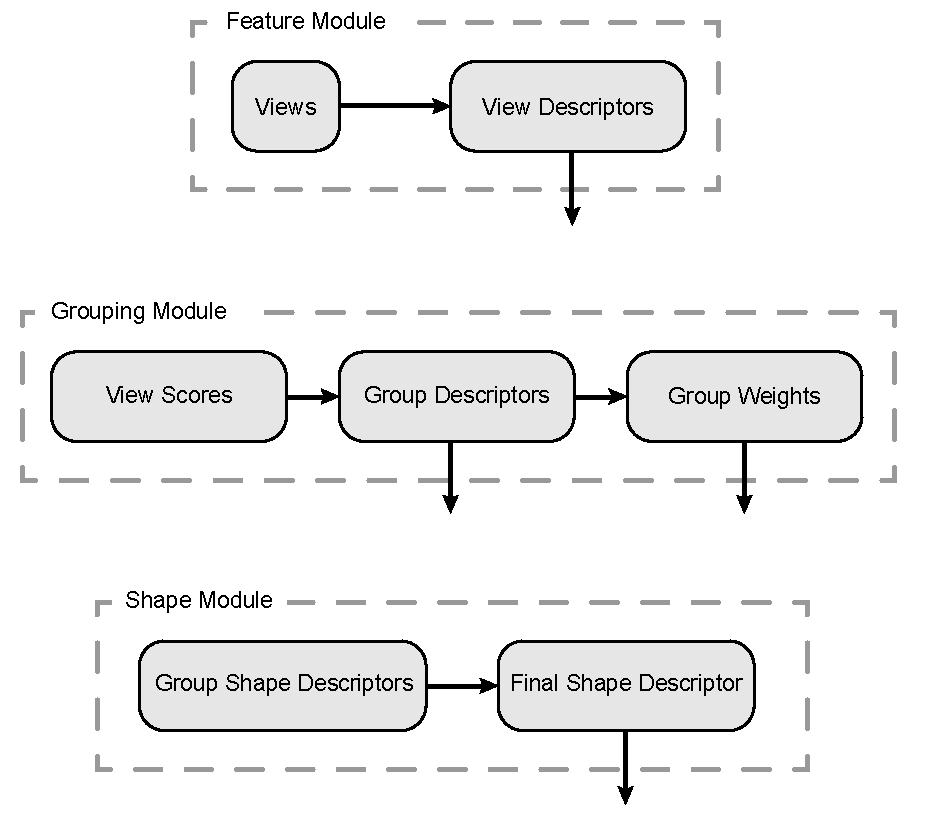
\includegraphics[]{images/multi_view_architecture.pdf}
	\caption{Modules of the multi-view architecture. The feature, grouping and shape modules are executed consecutively. Each module's operations are executed from left to right according their illustrated flow by arrows.}
	\label{fig:architecture-modules}
\end{figure}

\subsection{Feature Module: Generating View Descriptors}
\label{sec:architecture-feature-module}
The objective of the feature module is the generation of a descriptor for each view by using five convolutional layers.
Each one is referred to as a view descriptor $\vec{V}_i$ in the following.
\figref{fig:feature-module} shows the basic concept.
\begin{figure}
	\centering
	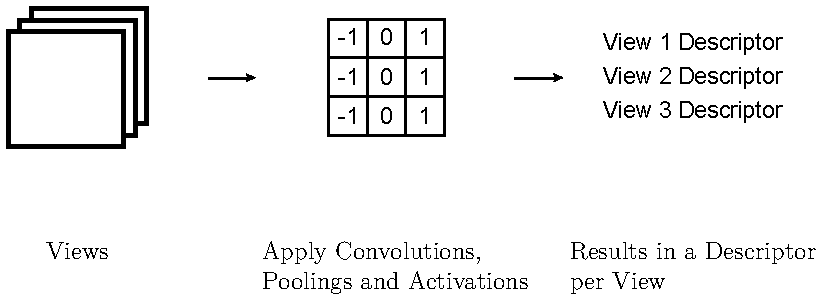
\includegraphics[]{images/feature_module.pdf}
	\caption{Basic Concept of the Feature Module}
	\label{fig:feature-module}
\end{figure}
This module is the first one in the feed-forward chain.
It is connected with the real world by having all views $\mathbb{V}$ of an object as its input.
Furthermore, because tensorflow supports batch execution, i.e. all its operations can be applied to a batch of data, the input tensor is extended with a batch dimension for multiple multi-views.
This yields an input tensor of shape $Batch \times Views \times Height \times Width \times Channels$.
In the following, if a tensor has a batch dimension, which is usually the case, it is assumed that any mentioned operation or approach is applied to every batch element.
This module consists of five main convolutional layers.
A main convolutional layer is supposed to have a convolutional layer and an optional pooling layer.
The first main layer performs a valid convolution with 96 filters of size $7 \times 7$ and a stride of 2 on each $224 \times 224 \times 3$ input.
Every filter extracts different features.
In comparison, the original AlexNet uses filters of size $11 \times 11$ and a stride of 4.
However, it is assumed that smaller filters and a smaller stride are collecting more information that can be used for a classification of the object and material at once.
A convolution operation is done by flattening the filter tensor to a 2D matrix of size $Filter\_Height \times Filter\_Width \times Channels\_In \times Channels\_Out$.
Here, $Channels\_in = 3$ because of the RGB channels of the input image and $Channels\_Out = 96$ because of the defined number of filters.
Then, image patches of shape $Batch \times Height\_Out \times Width\_Out \times Filter\_Height \cdot Filter\_Width \cdot Channels\_In$ are extracted from the input tensor.
Multiplying the filter matrix and the image patch vector yields the convolution results for the current window.
This is repeated for the whole input resulting in a matrix with a size of $1 \times 109 \times 109 \times 96$ in this case.
Furthermore, to each convolution output the corresponding bias is added.
This result is fed into a ReLU activation function.
Finally, the outputs are max-pooled with a window of size $3 \times 3$ and a stride of 2.
No padding is applied as well.
It is defined, that the max-pooling is always performed on the last dimension, i. e. the one containing each feature.
This yields a matrix of shape $1 \times 54 \times 54 \times 96$ for each convolution.
The next layers are similar including the bias addition and the ReLU activation function.
Hence, only the operations and their parameters will be mentioned.
Furthermore, the layers are added sequentially.
That means, the activations of the previous main layer are the input of the current main layer and so on.
The second main layer performs a convolution with 256 filters of size $5 \times 5$ and a stride of 2.
However, this time the input is padded in a way, that the output has the original input's size.
This yields a convolution result of shape $1 \times 27 \times 27 \times 256$.
The max-pooling uses again a window of $3 \times 3$ and a stride of 2.
The valid padding technique is applied resulting in a shape of $1 \times 13 \times 13 \times 256$.
The third and fourth main layer use 384 filters of size $3 \times 3$ for the convolution task with a stride of 1 each and the padding technique same.
However, no pooling is performed.
Hence, this yields a matrix of shape $1 \times 13 \times 13 \times 384$ both the times.
For the last main layer, the fifth one, a convolution with 256 filters of size $3 \times 3$ is performed.
The stride is 1 and the padding technique same, hence, the result has a size of $1 \times 13 \times 13 \times 256$.
The output's dimension is reduced with a valid max-pooling of size $3 \times 3$ and a stride of 2 to $1 \times 6 \times 6 \times 256$.
In the end, this whole process results in a tensor containing each view descriptor $\vec{V}_i$ of size $6 \times 6 \times 256$ of every batch element.
Hence, this tensor's shape is $Batch \times Views \times 6 \times 6 \times 256$.
\subsection{Grouping Module: Generating Group Descriptors}
\label{sec:architecture-grouping-module}
The objective of the grouping module is grouping each view descriptor $\vec{V}^{[5]}_v$ of an object depending on its information content.
This weights discriminative ones more than others, hence, improves the classification performance.
Moreover, based on each view's discrimination score an analysis of its information content is supported.
The view descriptors $\vec{V}^{[5]}_v$ of each group $\mathbb{G}_g$ are then combined to a group descriptor $\vec{G}_g$.
Hence, this module's inputs are the view descriptors coming from the feature module.
\begin{figure}
	\centering
	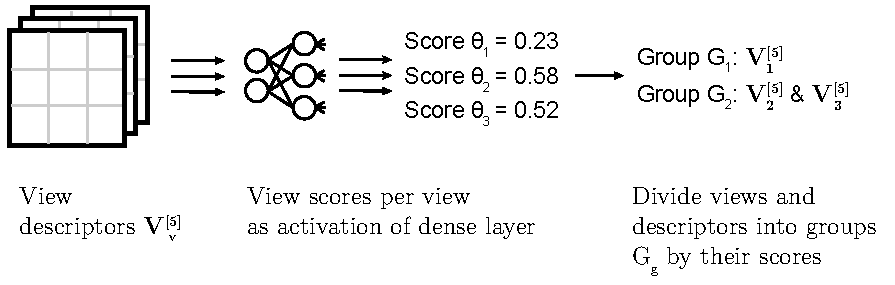
\includegraphics[]{images/grouping_module_groups.pdf}
	\caption{Group creation and view sorting in grouping module. Each view descriptor $\vec{V}^{[5]}_v$ is propagated through the same fully-connected layer yielding a view discrimination score $\theta_v$ based on which the view or view descriptor, respectively, is divided into a group $\mathbb{G}_g$.}
	\label{fig:grouping-module-groups}
\end{figure}
First, the informational content of each view needs to be calculated.
The simplest and most intuitive way is to give every view a single number representing its score of discrimination.
One approach would be to make the score directly depend on the pixel values.
This could be performed with a fully-connected layer with the pixels as inputs and the score as output.
However, like with fully-connected neural networks, this leads to many additional parameters for the network due to the translation-variance of input values. 
This could be overcome by using convolutions first for extracting features for the score.
However, discriminative features are already extracted, presumably much more accurate than a few convolutions for the score would do. 
Hence, the followed approach is that each view's score depends on its most recent descriptor $\vec{V}^{[5]}_v$.
It is worth noting, that in \cite{Feng2018} the view scores do not depend on the last convolution.
However, their network architecture uses more than five convolutional layers, but the scores depend on the fifth one as well.
This is probably because later features of deeper view descriptors are too detailed and would result in too divergent discrimination scores for a reliable group generation.
In this work's architecture each latest view descriptor $\vec{V}^{[5]}_v$ is fed into the same single fully-connected layer with one node.
Therefore, the view descriptor matrix is flattened into a row-wise vector, which is multiplied with the corresponding weight matrix $\vec{W}^{[d4]}$ of shape $6 \cdot 6 \cdot 256 \times 1$.
To this result a bias $b^{[d4]}$ is added yielding the weighted sum $z^{[d4]}$ with a single value.
This is fed into its activation function.
In contrast to every other layer in this network, a leaky ReLU activation function is applied to this unit.
A dropout is not performed, because with only one node it is not desirable.
Dropping out this node represents a view discrimination score of 0.
This would generalize the view scores way to strong, hence, unnecessarily extending training time.
Finding well-suited parameters for this layer would presumable take longer than for the others, thus, generating a bottle-neck in the architecture.
%It was found during training, that the unit died at the beginning of the training most of the time when using ReLU activation functions.
%This is due to its characteristic.
%If the weighted sum is zero or below at the beginning of the training due to an unsuited weight initialization, the activation is zero, hence, the neuron dies immediately.
%Another reason could be a too large learning rate, allowing the weights to update in too big steps leading to a weighted sum of 0 or below.
%This results in a view score of $0$ for every view that is not changed during later training steps due to a gradient of 0.
%The learning rate should suit the whole network and not only this layer, though.
%Their gradient is always unequal to zero, hence, it is solving the dying ReLU unit problem.

For interpretation purposes, the activation is squeezed into a range from 0 to 1 using the sigmoid function according to \cite{Feng2018} representing a probability of discrimination.
Because the sigmoid function saturates at values higher than around $\abs{5}$, but the activation of the fully-connected layer is assumed to be larger, the natural logarithm of the activation is computed first.
This shifts the saturation to values that are presumably not in the range of the activation.
For having a continuous function the absolute value of the activation is taken beforehand.
This yields the expression for a view's score
\begin{equation}
	\label{eq:view-discrimination-score}
	\theta_v = \sigmoid\left( \log \left( \abs{a^{[d4]}} + \varepsilon \right) \right)
\end{equation}
where $a^{[d4]}$ is the output or activation, respectively, of the corresponding fully-connected layer.
The small constant $\varepsilon=10^{-6}$ is added for numerical stability for avoiding $\log(0)$.
A plot of this function is shown in \figref{fig:view-discrimination-score}.
\begin{figure}
	\setlength\figureheight{.45\textwidth}
	\setlength\figurewidth{.8\textwidth}
	\centering
	% This file was created by matplotlib2tikz v0.7.4.
\begin{tikzpicture}

\begin{axis}[
height=\figureheight,
tick align=outside,
tick pos=left,
width=\figurewidth,
x grid style={white!90.01960784313725!black},
xlabel={Activation},
xmajorgrids,
xmin=-0.989, xmax=20.989,
xtick style={color=black},
y grid style={white!90.01960784313725!black},
ylabel={Discrimination Score},
ymajorgrids,
ymin=-0.0372218736880834, ymax=0.99948112962797,
ytick style={color=black},
ytick={-0.2,0,0.2,0.4,0.6,0.8,1},
yticklabels={−0.2,0.0,0.2,0.4,0.6,0.8,1.0}
]
\addplot [semithick, green!50.0!black]
table {%
0.01 0.0099009900990099
0.02 0.0196078431372549
0.03 0.029126213592233
0.04 0.0384615384615385
0.05 0.0476190476190476
0.06 0.0566037735849057
0.07 0.0654205607476635
0.08 0.0740740740740741
0.09 0.0825688073394495
0.1 0.0909090909090909
0.11 0.0990990990990991
0.12 0.107142857142857
0.13 0.115044247787611
0.14 0.12280701754386
0.15 0.130434782608696
0.16 0.137931034482759
0.17 0.145299145299145
0.18 0.152542372881356
0.19 0.159663865546219
0.2 0.166666666666667
0.21 0.173553719008264
0.22 0.180327868852459
0.23 0.186991869918699
0.24 0.193548387096774
0.25 0.2
0.26 0.206349206349206
0.27 0.21259842519685
0.28 0.21875
0.29 0.224806201550388
0.3 0.230769230769231
0.31 0.236641221374046
0.32 0.242424242424242
0.33 0.24812030075188
0.34 0.253731343283582
0.35 0.259259259259259
0.36 0.264705882352941
0.37 0.27007299270073
0.38 0.27536231884058
0.39 0.280575539568345
0.4 0.285714285714286
0.41 0.290780141843972
0.42 0.295774647887324
0.43 0.300699300699301
0.44 0.305555555555556
0.45 0.310344827586207
0.46 0.315068493150685
0.47 0.319727891156463
0.48 0.324324324324324
0.49 0.328859060402685
0.5 0.333333333333333
0.51 0.337748344370861
0.52 0.342105263157895
0.53 0.34640522875817
0.54 0.350649350649351
0.55 0.354838709677419
0.56 0.358974358974359
0.57 0.363057324840764
0.58 0.367088607594937
0.59 0.371069182389937
0.6 0.375
0.61 0.37888198757764
0.62 0.382716049382716
0.63 0.386503067484663
0.64 0.390243902439024
0.65 0.393939393939394
0.66 0.397590361445783
0.67 0.401197604790419
0.68 0.404761904761905
0.69 0.408284023668639
0.7 0.411764705882353
0.71 0.415204678362573
0.72 0.418604651162791
0.73 0.421965317919075
0.74 0.425287356321839
0.75 0.428571428571429
0.76 0.431818181818182
0.77 0.435028248587571
0.78 0.438202247191011
0.79 0.441340782122905
0.8 0.444444444444444
0.81 0.447513812154696
0.82 0.450549450549451
0.83 0.453551912568306
0.84 0.456521739130435
0.85 0.459459459459459
0.86 0.462365591397849
0.87 0.46524064171123
0.88 0.468085106382979
0.89 0.470899470899471
0.9 0.473684210526316
0.91 0.476439790575916
0.92 0.479166666666667
0.93 0.481865284974093
0.94 0.484536082474227
0.95 0.487179487179487
0.96 0.489795918367347
0.97 0.49238578680203
0.98 0.494949494949495
0.99 0.49748743718593
1 0.5
1.01 0.502487562189055
1.02 0.504950495049505
1.03 0.507389162561576
1.04 0.509803921568628
1.05 0.51219512195122
1.06 0.514563106796117
1.07 0.516908212560386
1.08 0.519230769230769
1.09 0.521531100478469
1.1 0.523809523809524
1.11 0.5260663507109
1.12 0.528301886792453
1.13 0.530516431924883
1.14 0.532710280373832
1.15 0.534883720930233
1.16 0.537037037037037
1.17 0.539170506912442
1.18 0.541284403669725
1.19 0.54337899543379
1.2 0.545454545454545
1.21 0.547511312217195
1.22 0.549549549549549
1.23 0.551569506726457
1.24 0.553571428571428
1.25 0.555555555555556
1.26 0.557522123893805
1.27 0.559471365638767
1.28 0.56140350877193
1.29 0.563318777292576
1.3 0.565217391304348
1.31 0.567099567099567
1.32 0.568965517241379
1.33 0.570815450643777
1.34 0.572649572649573
1.35 0.574468085106383
1.36 0.576271186440678
1.37 0.578059071729958
1.38 0.579831932773109
1.39 0.581589958158996
1.4 0.583333333333333
1.41 0.5850622406639
1.42 0.586776859504132
1.43 0.588477366255144
1.44 0.590163934426229
1.45 0.591836734693878
1.46 0.59349593495935
1.47 0.595141700404858
1.48 0.596774193548387
1.49 0.598393574297189
1.5 0.6
1.51 0.601593625498008
1.52 0.603174603174603
1.53 0.604743083003953
1.54 0.606299212598425
1.55 0.607843137254902
1.56 0.609375
1.57 0.610894941634241
1.58 0.612403100775194
1.59 0.613899613899614
1.6 0.615384615384615
1.61 0.616858237547893
1.62 0.618320610687023
1.63 0.619771863117871
1.64 0.621212121212121
1.65 0.622641509433962
1.66 0.62406015037594
1.67 0.625468164794008
1.68 0.626865671641791
1.69 0.628252788104089
1.7 0.62962962962963
1.71 0.6309963099631
1.72 0.632352941176471
1.73 0.633699633699634
1.74 0.635036496350365
1.75 0.636363636363636
1.76 0.63768115942029
1.77 0.63898916967509
1.78 0.640287769784173
1.79 0.6415770609319
1.8 0.642857142857143
1.81 0.644128113879004
1.82 0.645390070921986
1.83 0.646643109540636
1.84 0.647887323943662
1.85 0.649122807017544
1.86 0.65034965034965
1.87 0.651567944250871
1.88 0.652777777777778
1.89 0.653979238754325
1.9 0.655172413793104
1.91 0.656357388316151
1.92 0.657534246575343
1.93 0.658703071672355
1.94 0.659863945578231
1.95 0.661016949152542
1.96 0.662162162162162
1.97 0.663299663299663
1.98 0.664429530201342
1.99 0.665551839464883
2 0.666666666666667
2.01 0.667774086378738
2.02 0.66887417218543
2.03 0.66996699669967
2.04 0.671052631578947
2.05 0.672131147540984
2.06 0.673202614379085
2.07 0.674267100977199
2.08 0.675324675324675
2.09 0.676375404530744
2.1 0.67741935483871
2.11 0.678456591639871
2.12 0.679487179487179
2.13 0.680511182108626
2.14 0.681528662420382
2.15 0.682539682539683
2.16 0.683544303797468
2.17 0.684542586750789
2.18 0.685534591194969
2.19 0.686520376175549
2.2 0.6875
2.21 0.688473520249221
2.22 0.68944099378882
2.23 0.690402476780186
2.24 0.691358024691358
2.25 0.692307692307692
2.26 0.693251533742331
2.27 0.694189602446483
2.28 0.695121951219512
2.29 0.696048632218845
2.3 0.696969696969697
2.31 0.697885196374622
2.32 0.698795180722891
2.33 0.6996996996997
2.34 0.70059880239521
2.35 0.701492537313433
2.36 0.702380952380952
2.37 0.70326409495549
2.38 0.704142011834319
2.39 0.705014749262537
2.4 0.705882352941176
2.41 0.706744868035191
2.42 0.707602339181287
2.43 0.708454810495627
2.44 0.709302325581395
2.45 0.710144927536232
2.46 0.710982658959538
2.47 0.711815561959654
2.48 0.712643678160919
2.49 0.713467048710602
2.5 0.714285714285714
2.51 0.715099715099715
2.52 0.715909090909091
2.53 0.71671388101983
2.54 0.717514124293785
2.55 0.71830985915493
2.56 0.719101123595506
2.57 0.719887955182073
2.58 0.720670391061452
2.59 0.721448467966574
2.6 0.722222222222222
2.61 0.722991689750693
2.62 0.723756906077348
2.63 0.724517906336088
2.64 0.725274725274725
2.65 0.726027397260274
2.66 0.726775956284153
2.67 0.727520435967302
2.68 0.728260869565217
2.69 0.7289972899729
2.7 0.72972972972973
2.71 0.730458221024259
2.72 0.731182795698925
2.73 0.731903485254692
2.74 0.732620320855615
2.75 0.733333333333333
2.76 0.734042553191489
2.77 0.73474801061008
2.78 0.735449735449735
2.79 0.736147757255937
2.8 0.736842105263158
2.81 0.73753280839895
2.82 0.738219895287958
2.83 0.738903394255875
2.84 0.739583333333333
2.85 0.74025974025974
2.86 0.740932642487047
2.87 0.741602067183463
2.88 0.742268041237113
2.89 0.74293059125964
2.9 0.743589743589744
2.91 0.744245524296675
2.92 0.744897959183673
2.93 0.745547073791349
2.94 0.746192893401015
2.95 0.746835443037975
2.96 0.747474747474748
2.97 0.748110831234257
2.98 0.748743718592965
2.99 0.74937343358396
3 0.75
3.01 0.750623441396509
3.02 0.751243781094527
3.03 0.751861042183623
3.04 0.752475247524752
3.05 0.753086419753086
3.06 0.753694581280788
3.07 0.754299754299754
3.08 0.754901960784314
3.09 0.755501222493888
3.1 0.75609756097561
3.11 0.75669099756691
3.12 0.757281553398058
3.13 0.757869249394673
3.14 0.758454106280193
3.15 0.759036144578313
3.16 0.759615384615385
3.17 0.760191846522782
3.18 0.760765550239235
3.19 0.761336515513127
3.2 0.761904761904762
3.21 0.762470308788599
3.22 0.76303317535545
3.23 0.763593380614657
3.24 0.764150943396226
3.25 0.764705882352941
3.26 0.765258215962441
3.27 0.765807962529274
3.28 0.766355140186916
3.29 0.766899766899767
3.3 0.767441860465116
3.31 0.767981438515081
3.32 0.768518518518518
3.33 0.76905311778291
3.34 0.769585253456221
3.35 0.770114942528736
3.36 0.770642201834862
3.37 0.77116704805492
3.38 0.771689497716895
3.39 0.772209567198178
3.4 0.772727272727273
3.41 0.773242630385488
3.42 0.773755656108597
3.43 0.774266365688488
3.44 0.774774774774775
3.45 0.775280898876405
3.46 0.775784753363229
3.47 0.776286353467561
3.48 0.776785714285714
3.49 0.77728285077951
3.5 0.777777777777778
3.51 0.778270509977827
3.52 0.778761061946903
3.53 0.77924944812362
3.54 0.779735682819383
3.55 0.78021978021978
3.56 0.780701754385965
3.57 0.781181619256018
3.58 0.781659388646288
3.59 0.782135076252723
3.6 0.782608695652174
3.61 0.783080260303688
3.62 0.783549783549784
3.63 0.784017278617711
3.64 0.78448275862069
3.65 0.78494623655914
3.66 0.785407725321888
3.67 0.785867237687366
3.68 0.786324786324786
3.69 0.786780383795309
3.7 0.787234042553192
3.71 0.787685774946921
3.72 0.788135593220339
3.73 0.788583509513742
3.74 0.789029535864979
3.75 0.789473684210526
3.76 0.789915966386555
3.77 0.790356394129979
3.78 0.790794979079498
3.79 0.791231732776618
3.8 0.791666666666667
3.81 0.792099792099792
3.82 0.79253112033195
3.83 0.79296066252588
3.84 0.793388429752066
3.85 0.793814432989691
3.86 0.794238683127572
3.87 0.794661190965092
3.88 0.795081967213115
3.89 0.795501022494887
3.9 0.795918367346939
3.91 0.796334012219959
3.92 0.796747967479675
3.93 0.797160243407708
3.94 0.797570850202429
3.95 0.797979797979798
3.96 0.798387096774194
3.97 0.798792756539235
3.98 0.799196787148594
3.99 0.799599198396794
4 0.8
4.01 0.800399201596806
4.02 0.800796812749004
4.03 0.801192842942346
4.04 0.801587301587302
4.05 0.801980198019802
4.06 0.802371541501976
4.07 0.80276134122288
4.08 0.803149606299213
4.09 0.803536345776031
4.1 0.803921568627451
4.11 0.804305283757338
4.12 0.8046875
4.13 0.805068226120858
4.14 0.805447470817121
4.15 0.805825242718447
4.16 0.806201550387597
4.17 0.806576402321083
4.18 0.806949806949807
4.19 0.807321772639692
4.2 0.807692307692308
4.21 0.80806142034549
4.22 0.808429118773946
4.23 0.808795411089866
4.24 0.809160305343511
4.25 0.80952380952381
4.26 0.809885931558935
4.27 0.810246679316888
4.28 0.810606060606061
4.29 0.810964083175803
4.3 0.811320754716981
4.31 0.811676082862523
4.32 0.81203007518797
4.33 0.812382739212007
4.34 0.812734082397004
4.35 0.813084112149533
4.36 0.813432835820896
4.37 0.813780260707635
4.38 0.814126394052045
4.39 0.814471243042672
4.4 0.814814814814815
4.41 0.815157116451017
4.42 0.81549815498155
4.43 0.815837937384899
4.44 0.816176470588235
4.45 0.81651376146789
4.46 0.816849816849817
4.47 0.817184643510055
4.48 0.817518248175182
4.49 0.817850637522769
4.5 0.818181818181818
4.51 0.818511796733212
4.52 0.818840579710145
4.53 0.819168173598553
4.54 0.819494584837545
4.55 0.81981981981982
4.56 0.820143884892086
4.57 0.820466786355476
4.58 0.82078853046595
4.59 0.821109123434705
4.6 0.821428571428571
4.61 0.82174688057041
4.62 0.822064056939502
4.63 0.822380106571936
4.64 0.822695035460993
4.65 0.823008849557522
4.66 0.823321554770318
4.67 0.82363315696649
4.68 0.823943661971831
4.69 0.824253075571177
4.7 0.824561403508772
4.71 0.824868651488617
4.72 0.825174825174825
4.73 0.825479930191972
4.74 0.825783972125436
4.75 0.826086956521739
4.76 0.826388888888889
4.77 0.826689774696707
4.78 0.826989619377163
4.79 0.827288428324698
4.8 0.827586206896552
4.81 0.827882960413081
4.82 0.828178694158076
4.83 0.828473413379074
4.84 0.828767123287671
4.85 0.829059829059829
4.86 0.829351535836177
4.87 0.829642248722317
4.88 0.829931972789116
4.89 0.830220713073005
4.9 0.830508474576271
4.91 0.830795262267344
4.92 0.831081081081081
4.93 0.831365935919056
4.94 0.831649831649832
4.95 0.831932773109244
4.96 0.832214765100671
4.97 0.83249581239531
4.98 0.832775919732441
4.99 0.8330550918197
5 0.833333333333333
5.01 0.833610648918469
5.02 0.833887043189369
5.03 0.834162520729685
5.04 0.834437086092715
5.05 0.834710743801653
5.06 0.834983498349835
5.07 0.835255354200989
5.08 0.835526315789474
5.09 0.835796387520525
5.1 0.836065573770492
5.11 0.83633387888707
5.12 0.836601307189543
5.13 0.836867862969005
5.14 0.837133550488599
5.15 0.83739837398374
5.16 0.837662337662338
5.17 0.837925445705024
5.18 0.838187702265372
5.19 0.838449111470113
5.2 0.838709677419355
5.21 0.838969404186795
5.22 0.839228295819936
5.23 0.839486356340289
5.24 0.83974358974359
5.25 0.84
5.26 0.840255591054313
5.27 0.840510366826156
5.28 0.840764331210191
5.29 0.841017488076312
5.3 0.841269841269841
5.31 0.841521394611727
5.32 0.841772151898734
5.33 0.842022116903633
5.34 0.842271293375394
5.35 0.84251968503937
5.36 0.842767295597484
5.37 0.843014128728414
5.38 0.843260188087774
5.39 0.843505477308294
5.4 0.84375
5.41 0.84399375975039
5.42 0.844236760124611
5.43 0.84447900466563
5.44 0.84472049689441
5.45 0.844961240310077
5.46 0.845201238390093
5.47 0.845440494590417
5.48 0.845679012345679
5.49 0.845916795069337
5.5 0.846153846153846
5.51 0.846390168970814
5.52 0.846625766871166
5.53 0.846860643185299
5.54 0.847094801223242
5.55 0.847328244274809
5.56 0.847560975609756
5.57 0.84779299847793
5.58 0.848024316109423
5.59 0.848254931714719
5.6 0.848484848484849
5.61 0.848714069591528
5.62 0.848942598187311
5.63 0.849170437405732
5.64 0.849397590361446
5.65 0.849624060150376
5.66 0.84984984984985
5.67 0.850074962518741
5.68 0.850299401197605
5.69 0.850523168908819
5.7 0.850746268656716
5.71 0.85096870342772
5.72 0.851190476190476
5.73 0.851411589895988
5.74 0.851632047477745
5.75 0.851851851851852
5.76 0.85207100591716
5.77 0.852289512555391
5.78 0.852507374631268
5.79 0.852724594992636
5.8 0.852941176470588
5.81 0.853157121879589
5.82 0.853372434017595
5.83 0.853587115666179
5.84 0.853801169590643
5.85 0.854014598540146
5.86 0.854227405247813
5.87 0.854439592430859
5.88 0.854651162790698
5.89 0.854862119013062
5.9 0.855072463768116
5.91 0.855282199710565
5.92 0.855491329479769
5.93 0.855699855699856
5.94 0.855907780979827
5.95 0.856115107913669
5.96 0.85632183908046
5.97 0.856527977044476
5.98 0.856733524355301
5.99 0.856938483547926
6 0.857142857142857
6.01 0.85734664764622
6.02 0.857549857549858
6.03 0.857752489331437
6.04 0.857954545454546
6.05 0.858156028368794
6.06 0.858356940509915
6.07 0.858557284299859
6.08 0.858757062146893
6.09 0.858956276445698
6.1 0.859154929577465
6.11 0.859353023909986
6.12 0.859550561797753
6.13 0.859747545582048
6.14 0.859943977591036
6.15 0.86013986013986
6.16 0.860335195530726
6.17 0.860529986052999
6.18 0.860724233983287
6.19 0.860917941585535
6.2 0.861111111111111
6.21 0.86130374479889
6.22 0.861495844875346
6.23 0.861687413554634
6.24 0.861878453038674
6.25 0.862068965517241
6.26 0.862258953168044
6.27 0.862448418156809
6.28 0.862637362637363
6.29 0.862825788751715
6.3 0.863013698630137
6.31 0.863201094391245
6.32 0.863387978142077
6.33 0.863574351978172
6.34 0.863760217983651
6.35 0.863945578231293
6.36 0.864130434782609
6.37 0.864314789687924
6.38 0.86449864498645
6.39 0.86468200270636
6.4 0.864864864864865
6.41 0.865047233468286
6.42 0.865229110512129
6.43 0.865410497981157
6.44 0.865591397849462
6.45 0.865771812080537
6.46 0.865951742627346
6.47 0.866131191432396
6.48 0.866310160427808
6.49 0.86648865153538
6.5 0.866666666666667
6.51 0.866844207723036
6.52 0.867021276595745
6.53 0.867197875166003
6.54 0.86737400530504
6.55 0.867549668874172
6.56 0.867724867724868
6.57 0.867899603698811
6.58 0.868073878627968
6.59 0.868247694334651
6.6 0.868421052631579
6.61 0.868593955321945
6.62 0.868766404199475
6.63 0.868938401048493
6.64 0.869109947643979
6.65 0.869281045751634
6.66 0.869451697127937
6.67 0.869621903520209
6.68 0.869791666666667
6.69 0.869960988296489
6.7 0.87012987012987
6.71 0.87029831387808
6.72 0.870466321243523
6.73 0.870633893919793
6.74 0.870801033591731
6.75 0.870967741935484
6.76 0.871134020618557
6.77 0.871299871299871
6.78 0.87146529562982
6.79 0.871630295250321
6.8 0.871794871794872
6.81 0.871959026888604
6.82 0.872122762148338
6.83 0.872286079182631
6.84 0.872448979591837
6.85 0.872611464968153
6.86 0.872773536895674
6.87 0.872935196950445
6.88 0.873096446700508
6.89 0.873257287705957
6.9 0.873417721518987
6.91 0.873577749683944
6.92 0.873737373737374
6.93 0.873896595208071
6.94 0.874055415617128
6.95 0.874213836477987
6.96 0.874371859296482
6.97 0.874529485570891
6.98 0.87468671679198
6.99 0.874843554443054
7 0.875
7.01 0.875156054931336
7.02 0.875311720698254
7.03 0.87546699875467
7.04 0.875621890547264
7.05 0.875776397515528
7.06 0.875930521091811
7.07 0.876084262701363
7.08 0.876237623762376
7.09 0.876390605686032
7.1 0.876543209876543
7.11 0.876695437731196
7.12 0.876847290640394
7.13 0.8769987699877
7.14 0.877149877149877
7.15 0.877300613496933
7.16 0.877450980392157
7.17 0.877600979192167
7.18 0.877750611246944
7.19 0.877899877899878
7.2 0.878048780487805
7.21 0.878197320341048
7.22 0.878345498783455
7.23 0.878493317132442
7.24 0.878640776699029
7.25 0.878787878787879
7.26 0.878934624697337
7.27 0.879081015719468
7.28 0.879227053140097
7.29 0.879372738238842
7.3 0.879518072289157
7.31 0.879663056558363
7.32 0.879807692307692
7.33 0.879951980792317
7.34 0.880095923261391
7.35 0.880239520958084
7.36 0.880382775119617
7.37 0.8805256869773
7.38 0.880668257756563
7.39 0.880810488676996
7.4 0.880952380952381
7.41 0.881093935790725
7.42 0.881235154394299
7.43 0.881376037959668
7.44 0.881516587677725
7.45 0.881656804733728
7.46 0.881796690307329
7.47 0.881936245572609
7.48 0.882075471698113
7.49 0.882214369846879
7.5 0.882352941176471
7.51 0.882491186839013
7.52 0.882629107981221
7.53 0.882766705744431
7.54 0.882903981264637
7.55 0.883040935672515
7.56 0.883177570093458
7.57 0.883313885647608
7.58 0.883449883449883
7.59 0.883585564610012
7.6 0.883720930232558
7.61 0.883855981416957
7.62 0.883990719257541
7.63 0.884125144843569
7.64 0.884259259259259
7.65 0.884393063583815
7.66 0.884526558891455
7.67 0.884659746251442
7.68 0.884792626728111
7.69 0.884925201380898
7.7 0.885057471264368
7.71 0.885189437428243
7.72 0.885321100917431
7.73 0.88545246277205
7.74 0.88558352402746
7.75 0.885714285714286
7.76 0.885844748858448
7.77 0.885974914481186
7.78 0.886104783599089
7.79 0.886234357224118
7.8 0.886363636363636
7.81 0.886492622020431
7.82 0.886621315192744
7.83 0.886749716874292
7.84 0.886877828054299
7.85 0.887005649717514
7.86 0.887133182844244
7.87 0.887260428410372
7.88 0.887387387387387
7.89 0.887514060742407
7.9 0.887640449438202
7.91 0.887766554433221
7.92 0.887892376681614
7.93 0.888017917133259
7.94 0.888143176733781
7.95 0.888268156424581
7.96 0.888392857142857
7.97 0.888517279821628
7.98 0.888641425389755
7.99 0.888765294771969
8 0.888888888888889
8.01 0.889012208657048
8.02 0.889135254988914
8.03 0.889258028792912
8.04 0.889380530973451
8.05 0.889502762430939
8.06 0.88962472406181
8.07 0.889746416758545
8.08 0.889867841409692
8.09 0.88998899889989
8.1 0.89010989010989
8.11 0.890230515916575
8.12 0.890350877192982
8.13 0.890470974808324
8.14 0.890590809628009
8.15 0.890710382513661
8.16 0.890829694323144
8.17 0.890948745910578
8.18 0.891067538126362
8.19 0.891186071817193
8.2 0.891304347826087
8.21 0.8914223669924
8.22 0.891540130151844
8.23 0.891657638136511
8.24 0.891774891774892
8.25 0.891891891891892
8.26 0.892008639308855
8.27 0.892125134843581
8.28 0.892241379310345
8.29 0.892357373519914
8.3 0.89247311827957
8.31 0.892588614393126
8.32 0.892703862660944
8.33 0.892818863879957
8.34 0.892933618843683
8.35 0.893048128342246
8.36 0.893162393162393
8.37 0.893276414087513
8.38 0.893390191897655
8.39 0.893503727369542
8.4 0.893617021276596
8.41 0.893730074388948
8.42 0.893842887473461
8.43 0.893955461293743
8.44 0.894067796610169
8.45 0.894179894179894
8.46 0.894291754756871
8.47 0.894403379091869
8.48 0.894514767932489
8.49 0.894625922023182
8.5 0.894736842105263
8.51 0.89484752891693
8.52 0.894957983193277
8.53 0.895068205666317
8.54 0.89517819706499
8.55 0.895287958115183
8.56 0.895397489539749
8.57 0.895506792058516
8.58 0.895615866388309
8.59 0.895724713242961
8.6 0.895833333333333
8.61 0.895941727367326
8.62 0.896049896049896
8.63 0.896157840083074
8.64 0.896265560165975
8.65 0.896373056994819
8.66 0.89648033126294
8.67 0.896587383660807
8.68 0.896694214876033
8.69 0.896800825593395
8.7 0.896907216494845
8.71 0.897013388259526
8.72 0.897119341563786
8.73 0.897225077081192
8.74 0.897330595482546
8.75 0.897435897435897
8.76 0.897540983606557
8.77 0.897645854657114
8.78 0.897750511247444
8.79 0.897854954034729
8.8 0.897959183673469
8.81 0.898063200815494
8.82 0.89816700610998
8.83 0.898270600203459
8.84 0.898373983739837
8.85 0.898477157360406
8.86 0.898580121703854
8.87 0.898682877406282
8.88 0.898785425101215
8.89 0.898887765419616
8.9 0.898989898989899
8.91 0.899091826437941
8.92 0.899193548387097
8.93 0.899295065458207
8.94 0.899396378269618
8.95 0.899497487437186
8.96 0.899598393574297
8.97 0.899699097291876
8.98 0.899799599198397
8.99 0.8998998998999
9 0.9
9.01 0.9000999000999
9.02 0.900199600798403
9.03 0.900299102691924
9.04 0.900398406374502
9.05 0.900497512437811
9.06 0.900596421471173
9.07 0.900695134061569
9.08 0.900793650793651
9.09 0.900891972249752
9.1 0.900990099009901
9.11 0.90108803165183
9.12 0.901185770750988
9.13 0.901283316880553
9.14 0.90138067061144
9.15 0.901477832512315
9.16 0.901574803149606
9.17 0.901671583087512
9.18 0.901768172888016
9.19 0.901864573110893
9.2 0.901960784313726
9.21 0.90205680705191
9.22 0.902152641878669
9.23 0.902248289345064
9.24 0.90234375
9.25 0.902439024390244
9.26 0.902534113060429
9.27 0.902629016553067
9.28 0.90272373540856
9.29 0.902818270165209
9.3 0.902912621359223
9.31 0.903006789524733
9.32 0.903100775193798
9.33 0.903194578896418
9.34 0.903288201160542
9.35 0.903381642512077
9.36 0.903474903474903
9.37 0.903567984570878
9.38 0.903660886319846
9.39 0.903753609239654
9.4 0.903846153846154
9.41 0.903938520653218
9.42 0.904030710172745
9.43 0.904122722914669
9.44 0.904214559386973
9.45 0.904306220095694
9.46 0.904397705544933
9.47 0.904489016236867
9.48 0.904580152671756
9.49 0.90467111534795
9.5 0.904761904761905
9.51 0.904852521408183
9.52 0.904942965779468
9.53 0.905033238366572
9.54 0.905123339658444
9.55 0.90521327014218
9.56 0.90530303030303
9.57 0.905392620624409
9.58 0.905482041587902
9.59 0.905571293673277
9.6 0.90566037735849
9.61 0.905749293119698
9.62 0.905838041431262
9.63 0.905926622765757
9.64 0.906015037593985
9.65 0.906103286384977
9.66 0.906191369606004
9.67 0.906279287722587
9.68 0.906367041198502
9.69 0.90645463049579
9.7 0.906542056074766
9.71 0.906629318394024
9.72 0.906716417910448
9.73 0.906803355079217
9.74 0.906890130353817
9.75 0.906976744186046
9.76 0.907063197026022
9.77 0.907149489322191
9.78 0.907235621521336
9.79 0.907321594068582
9.8 0.907407407407408
9.81 0.907493061979648
9.82 0.907578558225508
9.83 0.907663896583564
9.84 0.907749077490775
9.85 0.907834101382488
9.86 0.907918968692449
9.87 0.908003679852806
9.88 0.908088235294118
9.89 0.908172635445363
9.9 0.908256880733945
9.91 0.908340971585701
9.92 0.908424908424908
9.93 0.908508691674291
9.94 0.908592321755027
9.95 0.908675799086758
9.96 0.908759124087591
9.97 0.908842297174111
9.98 0.908925318761384
9.99 0.909008189262966
10 0.909090909090909
10.01 0.909173478655767
10.02 0.909255898366606
10.03 0.909338168631006
10.04 0.909420289855073
10.05 0.909502262443439
10.06 0.909584086799277
10.07 0.9096657633243
10.08 0.909747292418773
10.09 0.909828674481515
10.1 0.90990990990991
10.11 0.90999099909991
10.12 0.910071942446043
10.13 0.91015274034142
10.14 0.910233393177738
10.15 0.910313901345291
10.16 0.910394265232975
10.17 0.91047448522829
10.18 0.910554561717352
10.19 0.910634495084897
10.2 0.910714285714286
10.21 0.910793933987511
10.22 0.910873440285205
10.23 0.910952804986643
10.24 0.911032028469751
10.25 0.911111111111111
10.26 0.911190053285968
10.27 0.911268855368234
10.28 0.911347517730496
10.29 0.911426040744021
10.3 0.911504424778761
10.31 0.91158267020336
10.32 0.911660777385159
10.33 0.911738746690203
10.34 0.911816578483245
10.35 0.911894273127753
10.36 0.911971830985915
10.37 0.912049252418646
10.38 0.912126537785589
10.39 0.912203687445127
10.4 0.912280701754386
10.41 0.912357581069237
10.42 0.912434325744308
10.43 0.912510936132983
10.44 0.912587412587413
10.45 0.912663755458515
10.46 0.912739965095986
10.47 0.9128160418483
10.48 0.912891986062718
10.49 0.912967798085292
10.5 0.91304347826087
10.51 0.913119026933102
10.52 0.913194444444444
10.53 0.913269731136167
10.54 0.913344887348354
10.55 0.913419913419913
10.56 0.913494809688581
10.57 0.913569576490925
10.58 0.913644214162349
10.59 0.913718723037101
10.6 0.913793103448276
10.61 0.913867355727821
10.62 0.91394148020654
10.63 0.914015477214102
10.64 0.914089347079038
10.65 0.914163090128755
10.66 0.914236706689537
10.67 0.914310197086547
10.68 0.914383561643836
10.69 0.914456800684346
10.7 0.914529914529915
10.71 0.914602903501281
10.72 0.914675767918089
10.73 0.914748508098892
10.74 0.914821124361158
10.75 0.914893617021277
10.76 0.914965986394558
10.77 0.915038232795242
10.78 0.915110356536503
10.79 0.915182357930449
10.8 0.915254237288136
10.81 0.91532599491956
10.82 0.915397631133672
10.83 0.915469146238377
10.84 0.91554054054054
10.85 0.915611814345991
10.86 0.915682967959528
10.87 0.91575400168492
10.88 0.915824915824916
10.89 0.915895710681245
10.9 0.915966386554622
10.91 0.916036943744752
10.92 0.916107382550336
10.93 0.91617770326907
10.94 0.916247906197655
10.95 0.916317991631799
10.96 0.916387959866221
10.97 0.916457811194653
10.98 0.91652754590985
10.99 0.916597164303586
11 0.916666666666667
11.01 0.916736053288926
11.02 0.916805324459235
11.03 0.916874480465503
11.04 0.916943521594684
11.05 0.91701244813278
11.06 0.917081260364842
11.07 0.917149958574979
11.08 0.917218543046358
11.09 0.917287014061208
11.1 0.917355371900826
11.11 0.917423616845582
11.12 0.917491749174918
11.13 0.917559769167354
11.14 0.917627677100494
11.15 0.917695473251029
11.16 0.917763157894737
11.17 0.917830731306491
11.18 0.917898193760263
11.19 0.917965545529122
11.2 0.918032786885246
11.21 0.918099918099918
11.22 0.918166939443535
11.23 0.918233851185609
11.24 0.918300653594771
11.25 0.918367346938776
11.26 0.918433931484502
11.27 0.918500407497962
11.28 0.9185667752443
11.29 0.918633034987795
11.3 0.91869918699187
11.31 0.91876523151909
11.32 0.918831168831169
11.33 0.91889699918897
11.34 0.918962722852512
11.35 0.919028340080972
11.36 0.919093851132686
11.37 0.919159256265158
11.38 0.919224555735057
11.39 0.919289749798224
11.4 0.919354838709677
11.41 0.91941982272361
11.42 0.919484702093398
11.43 0.919549477071601
11.44 0.919614147909968
11.45 0.919678714859438
11.46 0.919743178170144
11.47 0.919807538091419
11.48 0.919871794871795
11.49 0.919935948759007
11.5 0.92
11.51 0.920063948840927
11.52 0.920127795527157
11.53 0.920191540303272
11.54 0.920255183413078
11.55 0.920318725099602
11.56 0.920382165605096
11.57 0.920445505171042
11.58 0.920508744038156
11.59 0.920571882446386
11.6 0.920634920634921
11.61 0.920697858842189
11.62 0.920760697305864
11.63 0.920823436262866
11.64 0.920886075949367
11.65 0.920948616600791
11.66 0.921011058451817
11.67 0.921073401736385
11.68 0.921135646687697
11.69 0.921197793538219
11.7 0.921259842519685
11.71 0.9213217938631
11.72 0.921383647798742
11.73 0.921445404556167
11.74 0.921507064364207
11.75 0.92156862745098
11.76 0.921630094043887
11.77 0.921691464369616
11.78 0.921752738654147
11.79 0.921813917122752
11.8 0.921875
11.81 0.921935987509758
11.82 0.921996879875195
11.83 0.922057677318784
11.84 0.922118380062305
11.85 0.922178988326848
11.86 0.922239502332815
11.87 0.922299922299922
11.88 0.922360248447205
11.89 0.922420480993018
11.9 0.922480620155039
11.91 0.922540666150271
11.92 0.922600619195047
11.93 0.922660479505027
11.94 0.922720247295209
11.95 0.922779922779923
11.96 0.92283950617284
11.97 0.92289899768697
11.98 0.922958397534669
11.99 0.923017705927637
12 0.923076923076923
12.01 0.923136049192929
12.02 0.923195084485407
12.03 0.923254029163469
12.04 0.923312883435583
12.05 0.923371647509579
12.06 0.923430321592649
12.07 0.923488905891354
12.08 0.923547400611621
12.09 0.923605805958747
12.1 0.923664122137405
12.11 0.92372234935164
12.12 0.923780487804878
12.13 0.923838537699924
12.14 0.923896499238965
12.15 0.923954372623574
12.16 0.924012158054711
12.17 0.924069855732726
12.18 0.924127465857359
12.19 0.924184988627748
12.2 0.924242424242424
12.21 0.924299772899319
12.22 0.924357034795764
12.23 0.924414210128496
12.24 0.924471299093656
12.25 0.924528301886792
12.26 0.924585218702866
12.27 0.924642049736247
12.28 0.924698795180723
12.29 0.924755455229496
12.3 0.924812030075188
12.31 0.924868519909842
12.32 0.924924924924925
12.33 0.924981245311328
12.34 0.92503748125937
12.35 0.925093632958801
12.36 0.925149700598802
12.37 0.925205684367988
12.38 0.92526158445441
12.39 0.925317401045556
12.4 0.925373134328358
12.41 0.925428784489187
12.42 0.92548435171386
12.43 0.92553983618764
12.44 0.925595238095238
12.45 0.925650557620818
12.46 0.925705794947994
12.47 0.925760950259837
12.48 0.925816023738873
12.49 0.925871015567087
12.5 0.925925925925926
12.51 0.925980754996299
12.52 0.92603550295858
12.53 0.926090169992609
12.54 0.926144756277696
12.55 0.92619926199262
12.56 0.926253687315634
12.57 0.926308032424466
12.58 0.926362297496318
12.59 0.926416482707873
12.6 0.926470588235294
12.61 0.926524614254225
12.62 0.926578560939794
12.63 0.926632428466618
12.64 0.926686217008798
12.65 0.926739926739927
12.66 0.926793557833089
12.67 0.926847110460863
12.68 0.926900584795322
12.69 0.926953981008035
12.7 0.927007299270073
12.71 0.927060539752006
12.72 0.927113702623907
12.73 0.927166788055353
12.74 0.927219796215429
12.75 0.927272727272727
12.76 0.927325581395349
12.77 0.927378358750908
12.78 0.927431059506531
12.79 0.927483683828861
12.8 0.927536231884058
12.81 0.927588703837799
12.82 0.927641099855282
12.83 0.927693420101229
12.84 0.927745664739885
12.85 0.927797833935018
12.86 0.927849927849928
12.87 0.92790194664744
12.88 0.927953890489914
12.89 0.928005759539237
12.9 0.928057553956835
12.91 0.928109273903666
12.92 0.92816091954023
12.93 0.928212491026561
12.94 0.928263988522238
12.95 0.92831541218638
12.96 0.92836676217765
12.97 0.928418038654259
12.98 0.928469241773963
12.99 0.928520371694067
13 0.928571428571429
13.01 0.928622412562455
13.02 0.92867332382311
13.03 0.92872416250891
13.04 0.928774928774929
13.05 0.928825622775801
13.06 0.928876244665718
13.07 0.928926794598436
13.08 0.928977272727273
13.09 0.92902767920511
13.1 0.929078014184397
13.11 0.929128277817151
13.12 0.929178470254958
13.13 0.929228591648974
13.14 0.929278642149929
13.15 0.929328621908127
13.16 0.929378531073446
13.17 0.929428369795342
13.18 0.929478138222849
13.19 0.929527836504581
13.2 0.929577464788732
13.21 0.929627023223082
13.22 0.929676511954993
13.23 0.929725931131412
13.24 0.929775280898877
13.25 0.929824561403509
13.26 0.929873772791024
13.27 0.929922915206727
13.28 0.929971988795518
13.29 0.930020993701889
13.3 0.93006993006993
13.31 0.930118798043326
13.32 0.930167597765363
13.33 0.930216329378925
13.34 0.930264993026499
13.35 0.930313588850174
13.36 0.930362116991643
13.37 0.930410577592206
13.38 0.930458970792768
13.39 0.930507296733843
13.4 0.930555555555556
13.41 0.93060374739764
13.42 0.930651872399445
13.43 0.930699930699931
13.44 0.930747922437673
13.45 0.930795847750865
13.46 0.930843706777317
13.47 0.930891499654457
13.48 0.930939226519337
13.49 0.930986887508627
13.5 0.931034482758621
13.51 0.931082012405238
13.52 0.931129476584022
13.53 0.931176875430144
13.54 0.931224209078404
13.55 0.93127147766323
13.56 0.931318681318681
13.57 0.931365820178449
13.58 0.931412894375857
13.59 0.931459904043866
13.6 0.931506849315069
13.61 0.931553730321698
13.62 0.931600547195622
13.63 0.931647300068353
13.64 0.931693989071038
13.65 0.931740614334471
13.66 0.931787175989086
13.67 0.931833674164962
13.68 0.931880108991825
13.69 0.931926480599047
13.7 0.931972789115646
13.71 0.932019034670292
13.72 0.932065217391304
13.73 0.932111337406653
13.74 0.932157394843962
13.75 0.932203389830508
13.76 0.932249322493225
13.77 0.9322951929587
13.78 0.93234100135318
13.79 0.932386747802569
13.8 0.932432432432433
13.81 0.932478055367995
13.82 0.932523616734143
13.83 0.932569116655428
13.84 0.932614555256065
13.85 0.932659932659933
13.86 0.932705248990579
13.87 0.932750504371217
13.88 0.932795698924731
13.89 0.932840832773674
13.9 0.932885906040268
13.91 0.932930918846412
13.92 0.932975871313673
13.93 0.933020763563295
13.94 0.933065595716198
13.95 0.933110367892977
13.96 0.933155080213904
13.97 0.933199732798931
13.98 0.93324432576769
13.99 0.933288859239493
14 0.933333333333333
14.01 0.933377748167888
14.02 0.933422103861518
14.03 0.933466400532269
14.04 0.933510638297872
14.05 0.933554817275748
14.06 0.933598937583001
14.07 0.93364299933643
14.08 0.93368700265252
14.09 0.933730947647449
14.1 0.933774834437086
14.11 0.933818663136995
14.12 0.933862433862434
14.13 0.933906146728354
14.14 0.933949801849406
14.15 0.933993399339934
14.16 0.934036939313984
14.17 0.9340804218853
14.18 0.934123847167326
14.19 0.934167215273206
14.2 0.93421052631579
14.21 0.934253780407627
14.22 0.934296977660972
14.23 0.934340118187787
14.24 0.934383202099738
14.25 0.934426229508197
14.26 0.934469200524246
14.27 0.934512115258677
14.28 0.93455497382199
14.29 0.934597776324395
14.3 0.934640522875817
14.31 0.934683213585892
14.32 0.934725848563969
14.33 0.934768427919113
14.34 0.934810951760104
14.35 0.93485342019544
14.36 0.934895833333333
14.37 0.934938191281718
14.38 0.934980494148244
14.39 0.935022742040286
14.4 0.935064935064935
14.41 0.935107073329007
14.42 0.93514915693904
14.43 0.935191186001296
14.44 0.935233160621762
14.45 0.935275080906149
14.46 0.935316946959897
14.47 0.935358758888171
14.48 0.935400516795866
14.49 0.935442220787605
14.5 0.935483870967742
14.51 0.935525467440361
14.52 0.935567010309278
14.53 0.935608499678043
14.54 0.935649935649936
14.55 0.935691318327974
14.56 0.93573264781491
14.57 0.935773924213231
14.58 0.93581514762516
14.59 0.935856318152662
14.6 0.935897435897436
14.61 0.935938500960922
14.62 0.935979513444302
14.63 0.936020473448496
14.64 0.936061381074169
14.65 0.936102236421725
14.66 0.936143039591315
14.67 0.936183790682833
14.68 0.936224489795918
14.69 0.936265137029955
14.7 0.936305732484076
14.71 0.936346276257161
14.72 0.936386768447837
14.73 0.936427209154482
14.74 0.936467598475222
14.75 0.936507936507937
14.76 0.936548223350254
14.77 0.936588459099556
14.78 0.936628643852978
14.79 0.93666877770741
14.8 0.936708860759494
14.81 0.936748893105629
14.82 0.936788874841972
14.83 0.936828806064435
14.84 0.936868686868687
14.85 0.936908517350158
14.86 0.936948297604035
14.87 0.936988027725268
14.88 0.937027707808564
14.89 0.937067337948395
14.9 0.937106918238994
14.91 0.937146448774356
14.92 0.937185929648241
14.93 0.937225360954175
14.94 0.937264742785445
14.95 0.93730407523511
14.96 0.93734335839599
14.97 0.937382592360676
14.98 0.937421777221527
14.99 0.937460913070669
15 0.9375
15.01 0.937539038101187
15.02 0.937578027465668
15.03 0.937616968184654
15.04 0.937655860349127
15.05 0.937694704049844
15.06 0.937733499377335
15.07 0.937772246421904
15.08 0.937810945273632
15.09 0.937849596022374
15.1 0.937888198757764
15.11 0.937926753569212
15.12 0.937965260545906
15.13 0.938003719776813
15.14 0.938042131350682
15.15 0.938080495356037
15.16 0.938118811881188
15.17 0.938157081014224
15.18 0.938195302843016
15.19 0.938233477455219
15.2 0.938271604938272
15.21 0.938309685379395
15.22 0.938347718865598
15.23 0.938385705483672
15.24 0.938423645320197
15.25 0.938461538461538
15.26 0.93849938499385
15.27 0.938537185003073
15.28 0.938574938574939
15.29 0.938612645794966
15.3 0.938650306748466
15.31 0.93868792152054
15.32 0.938725490196078
15.33 0.938763012859767
15.34 0.938800489596083
15.35 0.938837920489297
15.36 0.938875305623472
15.37 0.938912645082468
15.38 0.938949938949939
15.39 0.938987187309335
15.4 0.939024390243902
15.41 0.939061547836685
15.42 0.939098660170524
15.43 0.939135727328059
15.44 0.939172749391727
15.45 0.939209726443769
15.46 0.939246658566221
15.47 0.939283545840923
15.48 0.939320388349515
15.49 0.939357186173439
15.5 0.939393939393939
15.51 0.939430648092065
15.52 0.939467312348668
15.53 0.939503932244404
15.54 0.939540507859734
15.55 0.939577039274924
15.56 0.939613526570048
15.57 0.939649969824985
15.58 0.939686369119421
15.59 0.939722724532851
15.6 0.939759036144578
15.61 0.939795304033715
15.62 0.939831528279182
15.63 0.939867708959711
15.64 0.939903846153846
15.65 0.93993993993994
15.66 0.939975990396159
15.67 0.94001199760048
15.68 0.940047961630695
15.69 0.94008388256441
15.7 0.940119760479042
15.71 0.940155595451825
15.72 0.940191387559809
15.73 0.940227136879856
15.74 0.94026284348865
15.75 0.940298507462687
15.76 0.940334128878282
15.77 0.940369707811568
15.78 0.940405244338498
15.79 0.940440738534842
15.8 0.940476190476191
15.81 0.940511600237954
15.82 0.940546967895363
15.83 0.94058229352347
15.84 0.94061757719715
15.85 0.940652818991098
15.86 0.940688018979834
15.87 0.9407231772377
15.88 0.940758293838863
15.89 0.940793368857312
15.9 0.940828402366864
15.91 0.940863394441159
15.92 0.940898345153664
15.93 0.940933254577673
15.94 0.940968122786305
15.95 0.941002949852507
15.96 0.941037735849057
15.97 0.941072480848556
15.98 0.941107184923439
15.99 0.941141848145968
16 0.941176470588235
16.01 0.941211052322163
16.02 0.941245593419507
16.03 0.94128009395185
16.04 0.94131455399061
16.05 0.941348973607038
16.06 0.941383352872216
16.07 0.941417691857059
16.08 0.941451990632319
16.09 0.941486249268578
16.1 0.941520467836257
16.11 0.941554646405611
16.12 0.941588785046729
16.13 0.941622883829539
16.14 0.941656942823804
16.15 0.941690962099125
16.16 0.941724941724942
16.17 0.94175888177053
16.18 0.941792782305006
16.19 0.941826643397324
16.2 0.941860465116279
16.21 0.941894247530506
16.22 0.941927990708478
16.23 0.941961694718514
16.24 0.94199535962877
16.25 0.942028985507246
16.26 0.942062572421784
16.27 0.942096120440069
16.28 0.94212962962963
16.29 0.942163100057837
16.3 0.942196531791907
16.31 0.942229924898902
16.32 0.942263279445728
16.33 0.942296595499134
16.34 0.942329873125721
16.35 0.942363112391931
16.36 0.942396313364055
16.37 0.942429476108232
16.38 0.942462600690449
16.39 0.942495687176538
16.4 0.942528735632184
16.41 0.942561746122918
16.42 0.942594718714122
16.43 0.942627653471027
16.44 0.942660550458716
16.45 0.94269340974212
16.46 0.942726231386025
16.47 0.942759015455066
16.48 0.94279176201373
16.49 0.942824471126358
16.5 0.942857142857143
16.51 0.942889777270131
16.52 0.942922374429224
16.53 0.942954934398175
16.54 0.942987457240593
16.55 0.943019943019943
16.56 0.943052391799544
16.57 0.943084803642573
16.58 0.943117178612059
16.59 0.943149516770893
16.6 0.943181818181818
16.61 0.943214082907439
16.62 0.943246311010216
16.63 0.943278502552467
16.64 0.943310657596372
16.65 0.943342776203966
16.66 0.943374858437146
16.67 0.943406904357668
16.68 0.943438914027149
16.69 0.943470887507066
16.7 0.943502824858757
16.71 0.943534726143422
16.72 0.943566591422122
16.73 0.943598420755781
16.74 0.943630214205186
16.75 0.943661971830986
16.76 0.943693693693694
16.77 0.943725379853686
16.78 0.943757030371204
16.79 0.943788645306352
16.8 0.943820224719101
16.81 0.943851768669287
16.82 0.94388327721661
16.83 0.943914750420639
16.84 0.943946188340807
16.85 0.943977591036415
16.86 0.944008958566629
16.87 0.944040290990487
16.88 0.94407158836689
16.89 0.944102850754612
16.9 0.94413407821229
16.91 0.944165270798437
16.92 0.944196428571429
16.93 0.944227551589515
16.94 0.944258639910814
16.95 0.944289693593315
16.96 0.944320712694878
16.97 0.944351697273233
16.98 0.944382647385984
16.99 0.944413563090606
17 0.944444444444444
17.01 0.94447529150472
17.02 0.944506104328524
17.03 0.944536882972823
17.04 0.944567627494457
17.05 0.944598337950139
17.06 0.944629014396456
17.07 0.944659656889873
17.08 0.944690265486726
17.09 0.944720840243228
17.1 0.94475138121547
17.11 0.944781888459415
17.12 0.944812362030905
17.13 0.944842801985659
17.14 0.944873208379272
17.15 0.944903581267218
17.16 0.944933920704846
17.17 0.944964226747386
17.18 0.944994499449945
17.19 0.94502473886751
17.2 0.945054945054945
17.21 0.945085118066996
17.22 0.945115257958288
17.23 0.945145364783324
17.24 0.945175438596491
17.25 0.945205479452055
17.26 0.945235487404162
17.27 0.945265462506842
17.28 0.945295404814004
17.29 0.945325314379442
17.3 0.945355191256831
17.31 0.945385035499727
17.32 0.945414847161572
17.33 0.94544462629569
17.34 0.945474372955289
17.35 0.945504087193461
17.36 0.945533769063181
17.37 0.945563418617311
17.38 0.945593035908596
17.39 0.945622620989668
17.4 0.945652173913043
17.41 0.945681694731124
17.42 0.9457111834962
17.43 0.945740640260445
17.44 0.945770065075922
17.45 0.94579945799458
17.46 0.945828819068256
17.47 0.945858148348674
17.48 0.945887445887446
17.49 0.945916711736074
17.5 0.945945945945946
17.51 0.945975148568342
17.52 0.946004319654428
17.53 0.946033459255262
17.54 0.946062567421791
17.55 0.946091644204852
17.56 0.946120689655172
17.57 0.946149703823371
17.58 0.946178686759957
17.59 0.946207638515331
17.6 0.946236559139785
17.61 0.946265448683503
17.62 0.946294307196563
17.63 0.946323134728932
17.64 0.946351931330472
17.65 0.946380697050938
17.66 0.946409431939979
17.67 0.946438136047134
17.68 0.946466809421841
17.69 0.94649545211343
17.7 0.946524064171123
17.71 0.946552645644041
17.72 0.946581196581197
17.73 0.9466097170315
17.74 0.946638207043757
17.75 0.946666666666667
17.76 0.946695095948827
17.77 0.946723494938732
17.78 0.946751863684771
17.79 0.946780202235232
17.8 0.946808510638298
17.81 0.946836788942052
17.82 0.946865037194474
17.83 0.946893255443441
17.84 0.94692144373673
17.85 0.946949602122016
17.86 0.946977730646872
17.87 0.947005829358771
17.88 0.947033898305085
17.89 0.947061937533086
17.9 0.947089947089947
17.91 0.947117927022739
17.92 0.947145877378436
17.93 0.947173798203909
17.94 0.947201689545934
17.95 0.947229551451187
17.96 0.947257383966245
17.97 0.947285187137586
17.98 0.947312961011591
17.99 0.947340705634544
18 0.947368421052632
18.01 0.947396107311941
18.02 0.947423764458465
18.03 0.947451392538098
18.04 0.947478991596639
18.05 0.94750656167979
18.06 0.947534102833158
18.07 0.947561615102255
18.08 0.947589098532495
18.09 0.947616553169199
18.1 0.947643979057592
18.11 0.947671376242805
18.12 0.947698744769874
18.13 0.947726084683743
18.14 0.947753396029258
18.15 0.947780678851175
18.16 0.947807933194154
18.17 0.947835159102765
18.18 0.947862356621481
18.19 0.947889525794685
18.2 0.947916666666667
18.21 0.947943779281624
18.22 0.947970863683663
18.23 0.947997919916797
18.24 0.948024948024948
18.25 0.948051948051948
18.26 0.948078920041537
18.27 0.948105864037364
18.28 0.948132780082988
18.29 0.948159668221877
18.3 0.948186528497409
18.31 0.948213360952874
18.32 0.94824016563147
18.33 0.948266942576306
18.34 0.948293691830403
18.35 0.948320413436693
18.36 0.948347107438017
18.37 0.94837377387713
18.38 0.948400412796698
18.39 0.948427024239299
18.4 0.948453608247423
18.41 0.948480164863472
18.42 0.948506694129763
18.43 0.948533196088523
18.44 0.948559670781893
18.45 0.948586118251928
18.46 0.948612538540596
18.47 0.948638931689779
18.48 0.948665297741273
18.49 0.948691636736788
18.5 0.948717948717949
18.51 0.948744233726294
18.52 0.948770491803279
18.53 0.948796722990271
18.54 0.948822927328557
18.55 0.948849104859335
18.56 0.948875255623722
18.57 0.948901379662749
18.58 0.948927477017365
18.59 0.948953547728433
18.6 0.948979591836735
18.61 0.949005609382968
18.62 0.949031600407747
18.63 0.949057564951605
18.64 0.94908350305499
18.65 0.94910941475827
18.66 0.949135300101729
18.67 0.949161159125572
18.68 0.949186991869919
18.69 0.94921279837481
18.7 0.949238578680203
18.71 0.949264332825977
18.72 0.949290060851927
18.73 0.94931576279777
18.74 0.949341438703141
18.75 0.949367088607595
18.76 0.949392712550607
18.77 0.949418310571573
18.78 0.949443882709808
18.79 0.949469429004548
18.8 0.94949494949495
18.81 0.949520444220091
18.82 0.949545913218971
18.83 0.949571356530509
18.84 0.949596774193548
18.85 0.949622166246851
18.86 0.949647532729104
18.87 0.949672873678913
18.88 0.949698189134809
18.89 0.949723479135244
18.9 0.949748743718593
18.91 0.949773982923154
18.92 0.949799196787149
18.93 0.949824385348721
18.94 0.949849548645938
18.95 0.949874686716792
18.96 0.949899799599198
18.97 0.949924887330996
18.98 0.94994994994995
18.99 0.949974987493747
19 0.95
19.01 0.950024987506247
19.02 0.95004995004995
19.03 0.950074887668497
19.04 0.950099800399202
19.05 0.950124688279302
19.06 0.950149551345962
19.07 0.950174389636273
19.08 0.950199203187251
19.09 0.950223992035839
19.1 0.950248756218905
19.11 0.950273495773247
19.12 0.950298210735587
19.13 0.950322901142573
19.14 0.950347567030784
19.15 0.950372208436725
19.16 0.950396825396825
19.17 0.950421417947447
19.18 0.950445986124876
19.19 0.950470529965329
19.2 0.950495049504951
19.21 0.950519544779812
19.22 0.950544015825915
19.23 0.950568462679189
19.24 0.950592885375494
19.25 0.950617283950617
19.26 0.950641658440276
19.27 0.950666008880118
19.28 0.95069033530572
19.29 0.950714637752588
19.3 0.950738916256158
19.31 0.950763170851797
19.32 0.950787401574803
19.33 0.950811608460403
19.34 0.950835791543756
19.35 0.950859950859951
19.36 0.950884086444008
19.37 0.950908198330879
19.38 0.950932286555446
19.39 0.950956351152526
19.4 0.950980392156863
19.41 0.951004409603136
19.42 0.951028403525955
19.43 0.951052373959863
19.44 0.951076320939335
19.45 0.951100244498778
19.46 0.951124144672532
19.47 0.951148021494871
19.48 0.951171875
19.49 0.95119570522206
19.5 0.951219512195122
19.51 0.951243295953193
19.52 0.951267056530214
19.53 0.951290793960058
19.54 0.951314508276534
19.55 0.951338199513382
19.56 0.95136186770428
19.57 0.951385512882839
19.58 0.951409135082604
19.59 0.951432734337057
19.6 0.951456310679612
19.61 0.95147986414362
19.62 0.951503394762367
19.63 0.951526902569074
19.64 0.951550387596899
19.65 0.951573849878935
19.66 0.951597289448209
19.67 0.951620706337687
19.68 0.951644100580271
19.69 0.951667472208797
19.7 0.951690821256039
19.71 0.951714147754708
19.72 0.951737451737452
19.73 0.951760733236855
19.74 0.951783992285439
19.75 0.951807228915663
19.76 0.951830443159923
19.77 0.951853635050554
19.78 0.951876804619827
19.79 0.951899951899952
19.8 0.951923076923077
19.81 0.951946179721288
19.82 0.951969260326609
19.83 0.951992318771003
19.84 0.952015355086372
19.85 0.952038369304556
19.86 0.952061361457335
19.87 0.952084331576425
19.88 0.952107279693487
19.89 0.952130205840115
19.9 0.952153110047847
19.91 0.952175992348159
19.92 0.952198852772467
19.93 0.952221691352126
19.94 0.952244508118434
19.95 0.952267303102625
19.96 0.952290076335878
19.97 0.952312827849308
19.98 0.952335557673975
19.99 0.952358265840877
};
\end{axis}

\end{tikzpicture}
	\caption{View discrimination score function plot}
	\label{fig:view-discrimination-score}
\end{figure}
All view discrimination scores for a batch are stored in a tensor $\bar{\vec{\Theta}}$ with shape $Batch \times Views$.

Dependent on each view score, the related views or view descriptors, respectively, are divided into groups.
For maximum flexibility, the number of groups $n_g$ equals the number of views $n_v$.
Hence, the size of each group bin $r_{\text{bin}}$ is related to the number of views $n_v$ per object and the range of possible view scores $r_\theta$.
With the limit of \eqref{eq:view-discrimination-score}
\begin{equation}
	\lim_{a^{[d4]}\rightarrow \infty} \sigmoid\left( \log \left( \abs{a^{[d4]}} + \varepsilon \right) \right) = 1
\end{equation}
and only positive values from the ReLU, scores are in the range $r_\theta = 1 - 0 = 1$.
Dividing $r_\theta$ in equal sized parts yields
\begin{equation}
	r_{\text{bin}} = \frac{r_\theta}{n_v} = \frac{1}{12} \approx 0.083
\end{equation}
as each group bin's size related to the discrimination score values.
Hence, a group $\mathbb{G}_g$ contains view descriptors $\vec{V}_v^{[5]}$ of views with scores of $(g-1) \cdot r_{\text{bin}} \leq \theta_v < g \cdot r_{\text{bin}}$ where $g \in \{1,2, \dots, n_v\}$.
\figref{fig:grouping-module-groups} illustrates the basic view score calculation and grouping.
This example assumes a group size of $0.33$.
The group to which each view $\tilde{\vec{X}}^{(i)}_v$ belongs is calculated by
\begin{equation}
	g_v = \floor \left( \frac{\vec{\theta}_v}{r_{\text{bin}}} \right)
\end{equation}
yielding the group's index, where $\vec{\theta}_v$ is the view score of the $v$-th view of the corresponding multi-view sample.
Those are stored for every view resulting in the group index vector $\vec{g}_{\text{idx}} = \left( g_1, g_2, \cdots, g_{n_v}\right)^T$.
The subscripts correspond to the view indices, e.g. $g_2$ belongs to $\tilde{\vec{X}}^{(i)}_2$.
With this approach, it is possible for groups to remain empty.
Based on the group indices, related view descriptors are averaged across their first dimension.
In brief, every feature is averaged.
This is illustrated in \figref{fig:grouping-module-group-descriptors}.
\begin{figure}
	\centering
	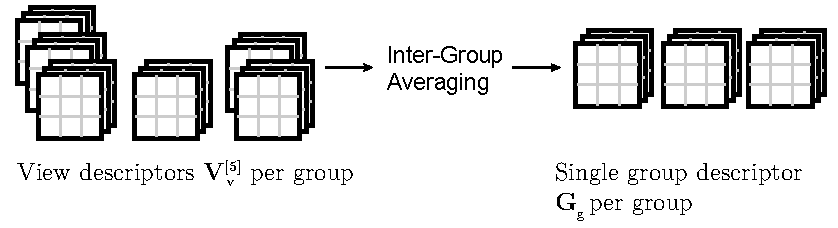
\includegraphics[]{images/grouping_module_group_descriptors.pdf}
	\caption[Generating group descriptors]{Generating group descriptors $\vec{G}_g$ by calculating the average of view descriptors $\vec{V}^{[5]}_v$ in each group $\mathbb{G}_g$.}
	\label{fig:grouping-module-group-descriptors}
\end{figure}
Because all view descriptors in a group should have similar extracted features, they can be combined by averaging them without a significant loss in information.
If the maximum of all features were taken, though, the group would presumably contain all view descriptors where important features were extracted for creating a group descriptor containing as many features as possible.
However, this is not desirable for the use case.
This results in a group descriptor
\begin{equation}
	\vec{G}_g = \frac{\sum_{\vec{D} \in \mathbb{G}_g} \vec{D}}{|\mathbb{G}_g|}
\end{equation}
with the same size as a view descriptor, where $\vec{D}$ is a view descriptor $\vec{V}_v^{[5]}$ of group $\mathbb{G}_g$.
The addition and division are calculated element-wise.
However, the views of different objects are not necessarily divided into the same number of groups, thus, leading to a different number of group descriptors.
For a valid matrix representation when using batches group descriptors of zero need to be added that the number of all batch's group descriptors match.
However, in the following $n_g$ is used for the group dimension for simplicity.
Hence, the final shape of the tensor $\bar{\vec{G}}$ containing all group descriptors is $Batch \times n_g \times 6 \times 6 \times 256$.

Every group $\mathbb{G}_g$ gets a weight $w_g$ assigned representing its discrimination.
This depends on the scores of its contained views.
Analog to before, views of a group are found by checking the group index vector $\vec{g}_{\text{idx}}$.
This time the related view scores are summed up and divided by their number for calculating a mean.
In mathematical terms,
\begin{equation}
	\hat{w}_g = \frac{\sum_{\vec{D} \in \mathbb{G}_g} \theta_v(\vec{D})}{|\mathbb{G}_g|}
\end{equation}
calculates the weight of the $g$-th group, where $\theta_v(\vec{D})$ is the score of a view descriptor $\vec{V}_v^{[5]}$ in $\mathbb{G}_g$.
Furthermore, the weight of a group is normalized by
\begin{equation}
	w_g = \frac{\hat{w}_g}{\max(\theta(\mathbb{G}_g))}
\end{equation}
to a range of 0 and 1, where $\max(\theta(\mathbb{G}_g))$ yields the maximum score of the given group, for being able to compare it with the ones in \cite{Feng2018}.
The calculation of the group weights is illustrated in \figref{fig:grouping-module-weights} referring to the example in \figref{fig:grouping-module-groups}.
\begin{figure}
	\centering
	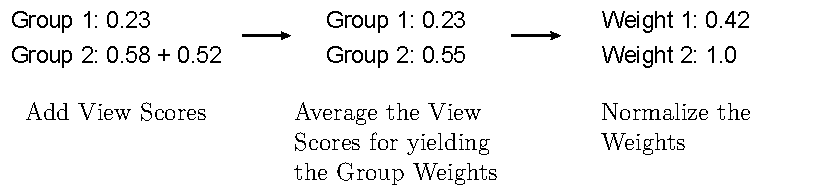
\includegraphics[]{images/grouping_module_weights.pdf}
	\caption{Calculation of group weights in grouping module}
	\label{fig:grouping-module-weights}
\end{figure}
All group weights of an object are stored in a vector $\vec{w}_{\text{groups}}$ of size $n_g$.
The corresponding tensor $\bar{\vec{W}}_{\text{groups}}$ has a size of $Batch \times n_g$.
\subsection{Shape Module: Generating a Shape Descriptor}
\label{sec:architecture-shape-module}
The objective of the shape module is to combine the group descriptors $\vec{G}_g$ of an object to a single shape descriptor that can be used for the classification.
All $n_g$ group descriptors of an object are stored in $\vec{G}$ that is of size $n_g \times 6 \times 6 \times 256$.
This descriptor contains every important feature of all views and groups.
Each group descriptor $\vec{G}_g$ is fed into a fully-connected sub-network with two layers.
The first layer has $6\cdot6\cdot256$ edges per unit and 4096 units in total, while the second layer has 4069 edges per unit and 4069 output units as well.
The inputs are processed like in the fully-connected layer before.
First, each input $\vec{G}_g$ is flattened into a column-vector $\vec{g}_g$.
Then, a matrix multiplication of the inputs and the corresponding weight matrix is performed and a bias vector is added.
This result is fed into a ReLU activation function $\phi(\cdot)$ resulting in an activation for the particular layer.
In conclusion, the two fully-connected operations
\begin{subequations}
	\begin{align}
		\vec{a}^{[6]}_g &= \phi(\vec{W}^{[6]} \vec{g}_g + \vec{b}^{[6]}) \\
		\vec{a}^{[7]}_g &= \phi(\vec{W}^{[7]} \vec{a}^{[6]}_g + \vec{b}^{[7]})
	\end{align}
\end{subequations}
are performed as illustrated in \figref{fig:shape-module-group-shape}.
\begin{figure}
	\centering
	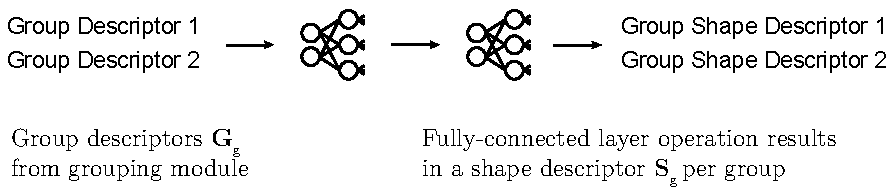
\includegraphics[]{images/shape_module_group_shape.pdf}
	\caption[Generate group shape descriptors in shape module]{Generate group shape descriptors in shape module. Each group descriptor $\vec{G}_g$ is propagated through two fully-connected layers representing layer 6 and 7 of the network. The activation of layer 7 represents the group shape descriptor $\vec{S}_g$ of each group descriptor.}
	\label{fig:shape-module-group-shape}
\end{figure}
Furthermore, both layers contain a dropout layer with a dropout probability of $0.5$.
This corresponds to the original AlexNet configuration.
Hence, the final activations of the seventh layer in the network or second dense layer, respectively, represent the shape descriptor of every group descriptor.
Those single group shape descriptor vectors of each group are and stacked along the second dimension to have a compact group shape descriptors representation $\vec{S}_{\text{groups}}$ with size $4096 \times n_g$.
Expanding this with a batch dimension yields the tensor $\bar{\vec{S}_{\text{groups}}}$ with size $Batch \times 4096 \times n_g$.

Now the group shape descriptors need to be combined for generating the final single shape descriptor of the object.
This is done by considering the corresponding group weights $\vec{w}_{\text{groups}}$ with $n_g$ elements calculated in the grouping module.
As a reminder, they are the mean of all view scores of each group, thus, an indicator for the group's discrimination.
Hence, a weighted average is calculated for considering this relation.
For this calculation the sums of the weights in inevitable.
Thus, $w_{g,\text{sum}}$ stores the sum of the group weights of an object.
The weighted average can be computed by
\begin{equation}
	\vec{s} = \frac{\vec{S}_{\text{groups}} \vec{w}_{\text{groups}}} {w_{\text{groups},\text{sum}}}
\end{equation}
where the division is performed element-wise.
The result has a shape of $4096$ and represents the final single shape descriptor.
The related assembled tensor $\bar{\vec{S}}$ has the size $Batch \times 4096$.

This representation is directly compatible with the last fully-connected layer, which is responsible for calculating the predictions of the network, thus, $\vec{s}$ is fed into it.
The number of neurons in this layer equals the number of classes where each neuron has 4096 edges.
The performed operations are identical to the ones earlier and are described by
\begin{equation}
	\vec{z}^{[8]} = \vec{W}^{[8]} \vec{s} + \vec{b}^{[8]}
\end{equation}
using the related weights and biases.
However, no activation function is applied here.
For making the predictions $\vec{z}^{[8]}$ interpretable, they are fed into a softmax layer.
This outputs a valid probability distribution $\hat{\vec{y}}$ depending on all its inputs $\vec{z}^{[8]}$.
Hence, this results in a membership probability for the network's input for each class.
The class representing the index with the largest value in $\hat{\vec{y}}$ is considered the predicted class. The functionality of the shape module is summarized in \figref{fig:shape-module-final-shape}.
\begin{figure}
	\centering
	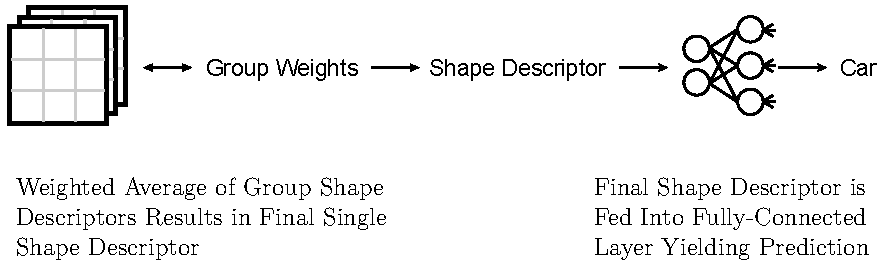
\includegraphics[]{images/shape_module_final_shape.pdf}
	\caption[Basic concept of the shape module]{Basic concept of the shape module combined with a classification. A weighted average of the group shape descriptors $\vec{S}_{\text{groups}}$ with the related group weights $w_{\text{groups}}$ is calculated yielding a single shape descriptor $\vec{s}$. It is fed into the last fully-connected layer resulting in the prediction $\hat{\vec{y}}$ of the network.}
	\label{fig:shape-module-final-shape}
\end{figure}
\section{Training the Architecture}
\label{sec:methods-training}
This work's multi-view network architecture is trained by inputting the generated multi-view images $\tilde{\vec{X}}_{train}^{(i)}$ and comparing the prediction $\hat{\vec{y}}^{(i)}$ of the network with the corresponding label $\tilde{\vec{y}}_{train}^{(i)}$.
First, a batch size needs to be chosen to define how many samples will be fed to the network at once.
In a training using only single-views, a batch size of 128 could be achieved.
Thus, using $n_v = 12$ views the batch size is reduced to $m_b = floor(128 / 12) = 10$.
However, due to a limited memory size of 8GB of the experimental setup's GPU and the additional parameters for the multi-view training only a batch size of 8 supports training reliably.
This yields $n_{b,train} = m_{train} / 8$ batches for the training set and $n_{b,test} = m_{test} / 8$ for the test set.
Nevertheless, dividing each set into 8 samples will be odd in general.
Thus, the last batch is filled with all the remaining samples.
After each epoch, the training set is shuffled randomly, so that batches do not contain the same samples as before.
For simplicity, a sample in the shuffled list is still referred to by its current index.

For calculating the cost and the derivatives of the parameters a softmax cross entropy is performed in the single-label classification case.
For efficiency, tensorflow applies a softmax internally, so the unscaled predictions need to be fed.
Then, the softmax measures the probability error between the prediction and ground-truth labels, while assuming mutually exclusive classes.
In the multi-label classification case, sigmoid cross entropy is applied.
Here the sigmoid is calculated internally and not mutually exclusive classes are assumed.
For updating the parameters with the goal of minimizing the cost function the Adam optimizer is employed due to its advantages.

The predictions $\hat{\bar{\tilde{\vec{Y}}}}^{(i)}$ of the network need to be compared to the ground-truth labels $\bar{\tilde{\vec{Y}}}^{(i)}$ of the $i$-th batch for checking the network's accuracy.
Due to the batch operations, the single dataset samples in a batch are referred to as batch samples.
How the comparison is performed, though, depends on the type of classification.
In the case of a single-label one, the index of the largest value in the batch element prediction $\hat{\tilde{\vec{y}}}^{(i)}$ is located.
The same operation is performed on the corresponding ground-truth label $\tilde{\vec{y}}^{(i)}$.
Each index represents a certain class, which is declared the predicted or actual one, respectively.
Now a binary comparison of both indices is performed, resulting in 0 if they are different and 1 if they are equal.
This is repeated for each batch element while storing all results in a tensor $\bar{\vec{E}}^{(i)}$.
Finally, the prediction accuracy $\alpha_{\text{p}}^{(i)}$ of the $i$-th batch is calculated by
\begin{equation}
	\label{eq:accuracy-mean}
	\alpha_{\text{p}}^{(i)} = \frac{\sum_{j} \bar{E}_j^{(i)}}{\left|\bar{\vec{E}}^{(i)}\right|}
\end{equation}
for the current batch $i$.
In the case of multi-label classification, a probability threshold needs to be defined when a predicted feature is actually considered predicted.
In this case, the threshold is $p_{\text{thres}}=0.5$, hence, the values of the prediction vector can be rounded.
Now an identical binary comparison as before can be applied to both label vectors resulting in a tensor $\bar{\vec{E}}^{(i)}$ as well.
The prediction accuracy is calculated with \eqref{eq:accuracy-mean}.

Furthermore, an initial learning rate is necessary.
Because finding it by trial-and-error would be time-consuming, the approach of the cyclical learning rate is used for finding an optimal learning rate.
The learning rate is initialized with $\gamma = 10^{-5}$.
After processing each batch it is exponentially increased according to
\begin{equation}
	\gamma(\tau+1) = \lambda \gamma(\tau)
\end{equation}
where $\lambda = 1.1$ is the scaling factor and $\tau$ the iteration.
Its value can be chosen arbitrarily but should be in range for achieving a desirable precision in learning rates.
For each learning rate, the related cost function evaluation is stored.
Training is stopped when the current cost value is four times the second to last one, i.\,e. when a drastic deterioration in cost happens, for having a noticeable oscillating characteristic at the end.
For evaluation, the cost values are plotted against the learning rates.
On the basis of this, the range of optimal learning rates can be read where a steep descent in cost values happen.
Optimally, this must be performed for each different network architecture.
\section{Evaluating the Architecture}
\label{sec:methods-evaluate}
For a comprehensive analysis of the network architecture of this work, especially the grouping mechanism and the information content of views, a lot of data has to be collected.
Fortunately, every tensor can be gathered and, if necessary, manipulated to be interpretable.
The most important tensor for training contains the cost of every iteration of the training set because this is attempted to be minimized, because it represents how well the network classifies the data.
Each one is stored during training to be able to plot them afterwards.
Furthermore, after each epoch, the cost and accuracy of the whole training and test set are calculated with current parameters.
Because the ModelNet10 dataset is split by default only into a training and test set, the latter is used additionally as a validation set.
The cost and accuracy of each set is computed by computing them for each batch and averaging the results.
However, the last batch has in general fewer elements than the ones before.
Hence, a weighted average is performed with the batch sizes as the weights.
This yields the averaged cost
\begin{equation}
	J\left(\hat{\bar{\tilde{\vec{Y}}}}, \bar{\tilde{\vec{Y}}}\right) =  \frac{\sum_{i}^{n_b} m_{b_i} \cdot J\left(\hat{\bar{\tilde{\vec{Y}}}}^{(i)}, \bar{\tilde{\vec{Y}}}^{(i)}\right)}{\left|\vec{m_b}\right|}
\end{equation}
and the averaged prediction accuracy
\begin{equation}
	\alpha_\text{p}\left(\hat{\bar{\tilde{\vec{Y}}}}, \bar{\tilde{\vec{Y}}}\right) =  \frac{\sum_{i}^{n_b} m_{b_i} \cdot \alpha_\text{p}\left(\hat{\bar{\tilde{\vec{Y}}}}^{(i)}, \bar{\tilde{\vec{Y}}}^{(i)}\right)}{\left|\vec{m_b}\right|}
\end{equation}
where $\vec{m_b}$ is a vector containing the batch sizes.
As mentioned, this is performed separately on the training set and the test set.
Those results are also stored for plotting purposes.
Comparing both related units can reveal if training should be continued or if overfitting or underfitting occurs.
Because the cost value is more general and the accuracy rather for practical purposes, the first one is examined.
If the training loss decreases while the training loss decreases as well, the network improves and training should be continued.
However, if the training loss decreases while the test loss increases, overfitting is indicated.
The network does not generalize, but focuses on the features in the training set, hence, never seen data like the test set cannot be classified properly.
At the end of the training, the accuracy of the training set is defined as the performance of the network.
To plots, whose shown values $\vec{\omega}$ oscillate, a moving average $\vec{\Omega}$ of the values is added.
A single averaged value is calculated by
\begin{equation}
	\Omega_i = \frac{\sum_{j = \max(1,i-\eta+1)}^{i} \omega_j}{\max(0,i-\eta)}
\end{equation}
where $\eta$ is the window size, that defines how many values are taken into account for averaging a certain sample.
If the window is larger than the available number of samples, in particular in the beginning, the window size is adapted temporarily.
By default it is set to $\eta=\floor\left( 0.1 \left| \vec{\omega} \right| \right)$ for a dynamical size.

For evaluating the whole network model regarding its practical use, the accuracies for each class, each category, and each color are calculated separately.
That means for the second and third, that each category accuracy includes all related multi-views independent of color and each color class accuracy includes all related multi-views independent of the category.
In general, the accuracy states how many samples are classified correctly.
However, the overall accuracy can be misleading, although each class has almost the same number of objects because it does not represent if certain classes are better classified than others.
Hence, the precision and recall score is computed for each class as well.
Furthermore, a simplified confusion matrix is calculated containing every sample's prediction.
It is plotted against the ground-truth classes, where predictions of identical classes are counted up.
The grouping module needs to be evaluated as well.
It is supposed that in a classification of only the color, the views with visible color manipulations belong to the highest weighted group.
Hence, it is sufficient to examine if the most discriminative group only contains views with visible manipulations.
Because the colors of the manipulated faces are known, each pixel of a view in the top group is checked if it matches such an RGB value.
If there is a match with at least one pixel of a view, the view is considered grouped correctly.
All correctly grouped views $TP$ and not correctly grouped views $FP$ are counted.
Based on them a percentage
\begin{equation}
	\label{eq:metric-group}
	\alpha_{\text{precision}}^{(i)} = \frac{{TP}^{(i)}}{{TP}^{(i)} + {FP}^{(i)}}
\end{equation}
is calculated representing the precision of the grouping module for a given multi-view input $i$.
This is repeated for all multi-views of the same color.
The final precision for that color results from averaging the precision of every multi-view of that color and is considered its group metric.
This is performed for every color to analyze if different colored face manipulations yield different results. 

For predicting the classes and gathering information of certain inputs, multi-views of objects need to be given.
These build a common input tensor $\bar{\tilde{\vec{X}}}^{(i)}$ representing the $i$-th batch.
If the number of samples, that are going to be predicted, exceeds the defined batch size, they need to be divided into an appropriate number of batches.
This tensor is now propagated through the network as usual.
%Meanwhile, the activations of the first convolutional layer are stored for visualizing the extracted features in each view.
%Therefore, each view's activations are split across the last dimension that represents the features.
%Each feature's values $\vec{F}_i$ are normalized by
%\begin{equation}
%	\label{eq:normalize}
%	\vec{F}_{i,norm} = \frac{\vec{F}_i - \min(\vec{F}_i)}{\max(\vec{F}_i) - \min(\vec{F}_i)} 
%\end{equation}
%to a range of 0 and 1 for making it visualizable.
%Finally, each feature is saved as an gray-scale image.
Meanwhile, each view discrimination score, group weight, and group index is stored for showing them with their associated view afterwards.
%Furthermore, a saliency map $\vec{S}_v^{(i)}$ is computed for each view $\tilde{\vec{X}}_v^{(i)}$ showing how much each pixel influences the raw output of the network $\vec{z}^{(i)}$.
%Here, the direct output of the eighth layer is taken, that means no softmax is applied.
%A single saliency map can be defined as the derivative of the output with respect to a single view yielding
%\begin{equation}
%	\label{eq:saliency-map}
%	\vec{S}_j^{(i)} = \frac{\partial \vec{z}^{(i)}}{\partial \tilde{\vec{X}}_v^{(i)}}
%\end{equation}
%as a general expression.
%For plotting each saliency map is normalized with \eqref{eq:normalize} and visualized in gray-scale.